\chapter{Incremental Dense Refinement}
\label{ch:incrDenseRef}
% \begin{mdframed}[hidealllines=true,backgroundcolor=blue!20]
The reconstruction method described in Chapter \ref{ch:manif}, builds a manifold mesh from a set of sparse data. 
The outcome captures the coarse geometry of the mesh, however, the reconstruction still lacks to capture the fine-grained details, even after the mesh sweeping proposed in Chapter \ref{ch:sweeping}.
In this chapter we aim at recovering the details of the geometry of the scene, incrementally, by means of variational optimization which directly evolves the surface of the scene according to images. 
We present a fully automatic pipeline to incrementally estimate the accurate reconstruction. 
In particular the method described is able to handle a multi-resolution mesh, and, instead of merging accurate submaps of the scene a posteriori and off-line, it combines online the reconstruction refined with the variational algorithm together with the new rough manifold estimated with the algorithms presented in the previous chapters.
% \end{mdframed}
\minitoc
\newpage

\section{Rationale}

Classical Multi-View Stereo methods \cite{gargallo2005bayesian,delaunoy_et_al_08} limits their application to batch processing and small-scale reconstructions.
The reasons are related both to the computational and memory resources needed to handle big set of images, and to the limitations of the optimization procedures that needs all the images at the same time.

In Chapter \ref{ch:soa} we saw that very few purely volumetric approaches have been proposed to incrementally build a model of the scene, as the algorithm proposed in this thesis (Chapter \ref{ch:manif}), or in \cite{lovi_et_al_11,hoppe2013incremental,litvinov_lhuillier_13}; however, as these algorithms are  only able to deal with sparse point and provide a rough recosntruction, not comparable to the \mvs results.

Recently, a very popular approach to  incremental dense reconstruction is based on depth maps\cite{pollefeys_et_al_08,collins1996space,newcombe2010live,ohtake2003multi,stuhmer2012parallel,stuckler2014multi} ; it first estimates the depth map for a selected set of keyframe, then it merges the depth maps into a single consistent 3D model of the scene, which usually relies on a voxel-based volumetric representation of the so called Truncated Signed-Distance Function (TDSF), therefore it is not suitable for large-scale reconstruction. 
Sch{\"o}ps \etal \cite{schops20153d} propose then to use voxel hashing together with a careful filtering of noisy depth data to deal with large scenes; the results are remarkable, but the resulting model is a non-continuous mesh, and the meshing step is not directly driven by the images, but by marching cubes \cite{lorensen1987marching} that interpolates the TSDF, as in most of the depth map based approaches.

Mesh-based algorithms represent an effective alternative to depth-maps and volumetric based reconstructions. Labatut \etal \cite{labatut2007efficient} estimate directly a visibility and photo-consistent mesh from the Delaunay triangulation of the 3D noisy points obtained from the depth maps.
Vu \etal  \cite{vu_et_al_2012} improve this algorithm by estimating an initial visibility-consistent mesh then by evolving the mesh such that it maximizes the photo-consistency with respect to the images. 
These Delaunay-based volumetric approaches are able to handle large scale scenes, but both \cite{labatut2007efficient} and \cite{vu_et_al_2012}  are not incremental.
Moreover, in the remarkable work of Vu \etal \cite{vu_et_al_2012}, the reconstruction pipeline   is not fully automatic, since  method proposed to estimate the initial mesh does not guarantee that manifold property holds for the whole model.



In this chapter we propose a framework to overcome the previous limitation and reconstruct a continuous and photo-consistent manifold mesh. 
We propose a fully automatic pipeline that integrates the method presented in the Chapter \ref{ch:manif}  with an accurate surface evolving refinement step applied incrementally thanks to a novel manifold-preserving mesh merging algorithm.


\section{System Overview}
 Our approach combines three steps  to provide a fully automatic and incremental reconstruction of the environment photo-consistent with the images. In Figure \ref{fig:architecture} we illustrate a scheme of the whole system. Every  $W$ frames the system outputs the available reconstruction.
 
 \begin{figure}[t]
  \centering
  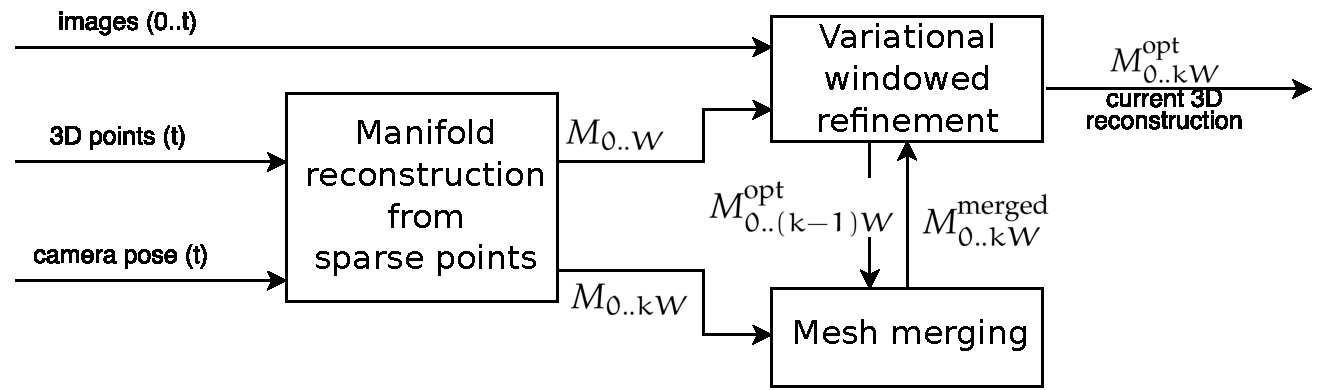
\includegraphics[width=0.9\textwidth]{./img/ch-incr-dens/incremental-mvs-architectureOK}
  \caption{Architecture of the parallel and incremental reconstruction system}
  \label{fig:architecture}
\end{figure}


The first step   builds incrementally a manifold mesh  from Structure from Motion 3D points and camera poses up to time $t$. We applied the algorithm described in Chapter \ref{ch:manif} that outputs a mesh $\mathit{M}_{0..t}$. The mesh  $\mathit{M}_{0..W}$ is a first rough initialization for the subsequent step. We combine all the subsequent meshes $\mathit{M}_{0..kW}$, with $k>1$, with the refined ones $\mathit{M}_{0..(k-1)W}^{\text{opt}}$. 
In this step we enforce the manifold property to consistently apply the mesh evolution process.
The second step is dedicated to the windowed variational refinement of the current mesh, which evolves the surface to maximize the photo-consistency between the last $W$ pairwise cameras.  
The output $\mathit{M}_{0..kW}^{\text{opt}}$ of this module is the current incremental optimized mesh, \ie, the output of the whole system.
%This approach reaches very accurate results and have been proved to scales well with large-scale scenes \cite{vu2011large}.
In the third step we merge the output of refinement, \ie,   $\mathit{M}_{0..(k-1)W}^{\text{opt}}$  and the new manifold $\mathit{M}_{0..kW}$ with a novel approach that keeps the manifold property and updates the topology. 
The output of this module is the multi-resolution mesh $\mathit{M}_{0..kW}^{\text{merged}}$ that feeds the refinement module.

% \begin{mdframed}[hidealllines=true,backgroundcolor=blue!20]
Let notice that this pipeline does not comprise the mesh sweeping algorithm proposed in Chapter \ref{ch:sweeping}; indeed, for a computational perspective, even if the mesh sweeping showed undeniable advantages, its implementation is still computational expensive compared to reconstruction from sparse points and mesh refinement.
However, incremental SfM applied to a subset of publicly available datasets we used, showed good reconstruction quality, such that we were able to refine the initial manifold without local minima issues.
% \end{mdframed}

In the following we describe the refinement and the merging step since the incremental manifold reconstruction from the sparse points of the Structure from motion, is described in Chapter \ref{ch:manif}.

\section{Windowed variational refinement}
\label{sec:Incremental_photoconsistent}
Whenever a manifold mesh that represents roughly the observed scene is available (see Chapter \ref{ch:manif}), we refine it in order to minimize the photo-metric error between pairwise camera induced by reconstructed surface. 
The approach adopted in our system is framed into the variational problem of finding a convenient function (the reconstructed surface) that  accurately represents the image data.
The variation of an energy function $E$ induced by a vector field $v$ on a surface $\mathit{S}$, leads to the functional gradient
\begin{equation}
\label{eq::calculus}
 DE(\mathit{S})_v = \left.\frac{\partial E(\mathit{S} + \epsilon v)}{\partial \epsilon} \right|_{\epsilon=0} = \int_{\mathit{S}} \nabla E(x)v(x) dx.
\end{equation}

Our surface refinement algorithms minimize an energy:
\begin{equation}
\label{eq:en}
E = E_{\textrm{photo}} + E_{\textrm{smooth}} ,
\end{equation}
where  $E_{\textrm{photo}}$ represents the energy induced by photo-consistency with the images, and $E_{\textrm{smooth}}$ is a prior energy that usually enforce the smoothness of the surface.  
We first describe how we minimize the first term which encodes the photo-consistency.

Let consider two images $I$ and $J$, and the surface reconstructed $\mathit{S}$ (our mesh). Let $x$ and $\overrightarrow{n}$ be a point on this surface and the corresponding normal. 
We define a function $err^S_{I, J}(x_i,\overrightarrow{n})$ which is the photo-metric similarity measure defined on the surface domain, and a visibility function $v^{\mathit{S}}_{ij}(x)$ that is equal to 1 where the surface is visible from both $I$ and $J$, otherwise is 0. 
In the early approach of Faugeras \etal \cite{faugeras2002variational} the energy $E_{\textrm{photo}}$ is integrated on the surface, and becomes:
\begin{equation}
 E_{\textrm{photo}} = \sum_{i,j}\int_{\mathit{S}} v^{\mathit{S}}_{ij}(x) err^S_{I,J}(x_i, \overrightarrow{n}) d\mathit{S}
\end{equation}


In our case we prefer to minimize  over the images, as in \cite{pons2007multi}, such that we rely directly on the data.
The function $err^S_{I, J}(x_i,\overrightarrow{n})$ becomes 
$err_{I, J}(x_i)$ that decreases if the similarity between the patch around the projection of $x_i$ in  $J$ and $I$ increases.
The energy $E_{\textrm{photo}}$ in Equation \eqref{eq:en} becomes:
\begin{equation}
\label{eq:energy_photo}
  E_{\textrm{photo}} = \sum_{i,j}\int_{\Omega^{\textrm{S}}_{i,j}} err_{I, I_{ij}^{\mathit{S}}}(x_i)\textrm{d}x_i = \sum_{i,j} \mathit{err}^{int}_{ij}(x)
\end{equation}
where the term $I_{ij}^{\mathit{S}}$ represents the reprojection of the image from the $j$-th camera in the image $I$ through the surface $\mathit{S}$
(Figure \ref{fig:cameraproj}).
The reasons to choose the latter energy are twofold: we do not explicilty need to consider the visibility and we directly compare the images in their natural domain.

Classical approaches in Computer Vision both in surface evolution and in other reconstruction methods, such as voxel-based ones, optimize the energy over a continuous representation of the surface then they discretize the minimizing flow to evolve the mesh-based representation \cite{pons2007multi,faugeras2002variational}. Recently a more coherent approach shows better results \cite{vu_et_al_2012,delaunoy_et_al_08}: it is named discretize-then-optimize and it directly takes into account the mesh representation during the optimizing procedure. 
Therefore we now modify Equation \eqref{eq::calculus} in order to take into account that  surface $\mathit{S}$ is represented by a triangular mesh.

Let $X_i \in \mathbb{R}^3$ be a mesh vertex. The discrete vector field $v$ associates to each $i$-th vertex a vector $v_i$ defined such that $v(x) = \sum_i \phi_i(x) v_i$, where $\phi_i(x)$ are the barycentric coordinates if $x$ is in the triangle containing $X_i$, then,  otherwise $\phi_i(x) = 0$ (in Appendix \ref{app:barycentric_} we explain barycentric coordinates).


\begin{figure}[t]
\centering
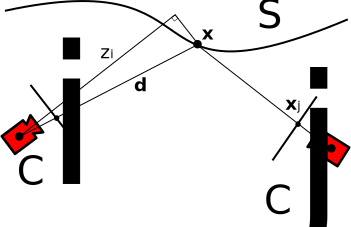
\includegraphics[width=0.92\textwidth]{./img/ch-incr-dens/cameproj}
\caption{Variables involved in the photometric refinement process}.
\label{fig:cameraproj}
\end{figure}

The Equation \eqref{eq::calculus} of the gradient functional becomes:
\begin{equation}
  DE(\mathit{S})_v = \sum_i v_i \int_{\mathit{S}} \phi_i(x) \nabla E(x) \textrm{d}x.
\end{equation}

And the discrete version of this gradient computed for a single vertex of the mesh becomes:
\begin{equation}
  \frac{\textrm{d}E(\mathit{S})}{\textrm{d}X_i} =  \int_{\mathit{S}} \phi_i(x) \nabla E(x) \textrm{d}x.
\end{equation}

In our case we need to compute the gradient of the energy defined in Equation \eqref{eq:energy_photo}:
\begin{equation}
  \nabla E_{\textrm{photo}} = \nabla (\sum_{i,j} err^{int}_{ij}(x)) = \sum_{i,j} \nabla err^{int}_{ij}(x).
\end{equation}
Let's suppose the point $x$ projects in points $x_i = \Pi_i(x) \in I_i$ and  $x_j = \Pi_j(x) \in I_j$, then, the vector $\mathbf{d}_i$ goes from camera $i$ to point $x$, $z_i$ is the depth of $x$ in camera $i$, and $\overrightarrow{n}$ is the normal at $x$ pointing outward the surface $\mathit{S}$. 
With the change of variable $\textrm{d}x_i = -\overrightarrow{n}^T \mathbf{d}_i \textrm{d}x/z_i^3$ (see Appendix \ref{app:change}):
\begin{align}
 \begin{split}
  \nabla err^{int}_{ij}(x)& = \\
  &=-\overrightarrow{n} \left( \partial_2 err_{I_i, I_{ij}^{\mathit{S}}}(x_i) DI_j(x_j) D\Pi_j(x)\frac{\mathbf{d}_i}{z_i^3}\right)=\\
  &= - f_{ij}(x_i) \overrightarrow{n}/z_i^3.
 \end{split}
\end{align}
    
where operator $D$ represents the derivative and $\partial_2 err_{I_i, I_{ij}^{\mathit{S}}}(x_i)$ is the derivative of $err_{ij}(x)$ with respect to the second image.


We then are able to rewrite the discrete gradient:
\begin{equation}
  \frac{\textrm{d}E(\mathit{S})}{\textrm{d}X_i} =  - \int_{\mathit{S}} \phi_i(x) \sum_{i,j} \nabla err^{int}_{ij}(x) \textrm{d}x 
\end{equation}

\begin{equation}
  =  - \sum_{i,j} \int_{\mathit{S}} \phi_i(x)  f_{ij}(x_i)  \overrightarrow{n}/z_i^3 \textrm{d}x 
\end{equation}
\begin{equation}
\label{eq:final}
  =  - \sum_{i,j} \int_{\mathit{S}} \phi_i(x)  f_{ij}(x_i)  \overrightarrow{n}/z_i^3 \frac{z_i^3}{\overrightarrow{n}^T \mathbf{d}_i }\overrightarrow{n} \textrm{d}x_i
\end{equation}
% 
% \begin{equation}
% \label{eq:final}
%   =  - \sum_{i,j} \int_{{\Omega_{i,j}}} \phi_i(x)  f_{ij}(x_i)  \overrightarrow{n}/z_i^3 \frac{z_i^3}{\overrightarrow{n}^T \mathbf{d}_i }\overrightarrow{n} \textrm{d}x_i
% \end{equation}

where $\Omega_{i,j}$ represents the surface region that induces the projection of image $I_j$ into the image $I_i$.
The summation in \eqref{eq:final} can be applied incrementally to the subset of the whole images according to those viewing the current mesh $M_{0..t}^{\text{merged}}$.

On the other hand, we minimize the energy $E_{\textrm{smooth}}$ as in \cite{vu_et_al_2012} by means of the Laplace-Beltrami operator approximated with the umbrella operator \cite{wardetzky2007discrete}, which moves each vertex in the mean position of its neighbors (see Section \ref{sec:sm}).

During this iterative process we increase the resolution of the mesh through One-to-four midpoint subdivision algorithm (Section \ref{sec:onefour}) until a triangle project in each images with an area smaller than 16 pixels.

% \begin{mdframed}[hidealllines=true,backgroundcolor=blue!20]
\subsection{Implementation Details}
The photometric refinement highly rely on GPU processing; we use OpenGL library \cite{opengl} and the GLSL shaders. As shown in Section \ref{sec:opengl_sweep} OpenGL natively manage the projection of one image to another through a model by means of texturing and rendering processes.

In Figure \ref{fig:openglIncrRef} we illustrate how we implemented the photometric refinement, of a mesh $\mathit{M}$ with respect to two images $I_{1}$ and $I_{2}$ captured by $C_{1}$ and $C_{2}$.
As a first step we send $\mathit{M}$  to  the GPU; we compute the depth of the mesh from the two point of view of camera $C_{1}$ and $C_{2}$ to define the visibility (\emph{Depth} block).
We project $I_{2}$ to the model and we render it to $C_{1}$ (\emph{Reprojection} block) and we compare this projection with the original image $I_{1}$ captured by camera $C_{1}$ to compute the NCC, the block-wise mean and variance  in a $5x5$ px neighborhood (\emph{NCC} block).
The outputs are needed to compute the $\partial_2 err_{I_i, I_{ij}^{\mathit{S}}}(x_i)$ (\emph{Similarity Gradient} block), which in turn is used to compute per-pixel $f_{ij}(x_i)  \overrightarrow{n}/z_i^3 \frac{z_i^3}{\overrightarrow{n}^T \mathbf{d}_i }\overrightarrow{n}$ of Equation \eqref{eq:final} (\emph{Gradient Flow} block). 
Finally, for each vertex, we finally collect the contributions over each incident triangle (\emph{Collect Gradient} block); we apply the resulting vector to the vertex and we compute its new position.

% \end{mdframed}
\begin{figure}[tp]
\centering
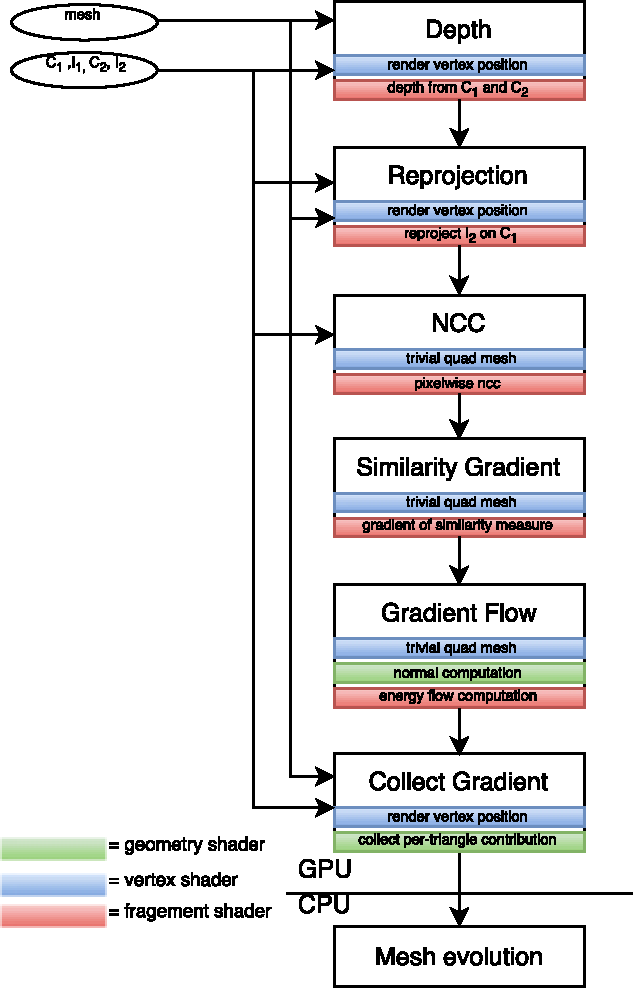
\includegraphics[height=0.92\textheight]{./img/ch-incr-dens/incr-shaders-architecture}
\caption{Architecture of the photometric algorithm.}
\label{fig:openglIncrRef}
\end{figure}


\section{Manifold-preserving Mesh Stitching}
\label{sec:Mesh_merging}
In the proposed system we need to merge the manifold mesh reconstructed incrementally with the mesh after the refinement.
We propose a novel merging approach, different from existing methods such as \cite{turk1994zippered} and \cite{VuPhD011} which deal with meshes with similar resolution and significant overlap. 
In particular  Vu  \cite{VuPhD011} merges together two  refined mesh; the,  he re-triangulates the overlapping areas and he stitches the borders through graph cut-algorithm over the 3D Constrained Delaunay triangulation of the border edges.
This approach only merges similar resolution and good overlapping meshes, it fixes a posteriori the non-manifoldnesses, and, the surface evolution refinement is not directly applied to the stitched areas.


In our case, in order to incrementally reconstruct and refine the whole mesh, we need to attach the missing part of the scene as soon as a new rough reconstruction is available. Therefore we propose a new approach to merge two meshes with  different resolutions, \ie, the refined and the rough meshes, such that, when they overlap, we  keep the refined part and reject the rough one.
After such multi-resolution merging step the algorithm described in the previous section is able to jointly refine both the newly added region together with the refined part.

The main idea of our mesh merging is to select a subregion of the refined and the new meshes such that by joining  the boundaries we keep the manifold property valid.
Let $\mathit{M}$ and  $\mathit{M}^{\text{opt}}$ be the new manifold and the refined mesh, \eg, blue and green meshes in Figure \ref{fig:mesh_merging}(a). 
% Let  $f_j \in \mathit{M}$ and $f_i^{\text{opt}} \in \mathit{M}^{\text{opt}}$ be the facets of the two mesh.




\begin{figure}[tpb]
\centering
\setlength{\tabcolsep}{1px}
\begin{tabular}{cc}
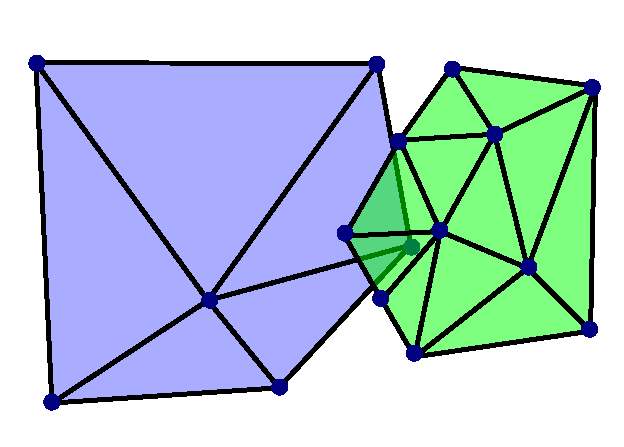
\includegraphics[width=0.475\textwidth]{./img/ch-incr-dens/meshmerge01new}&
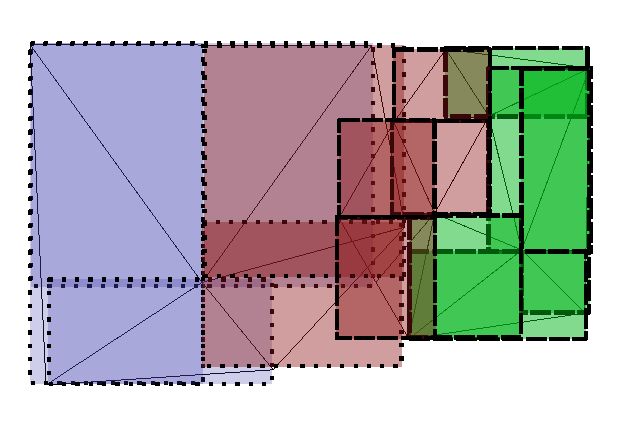
\includegraphics[width=0.475\textwidth]{./img/ch-incr-dens/meshmerge02new}\\
(a)&(b)\\
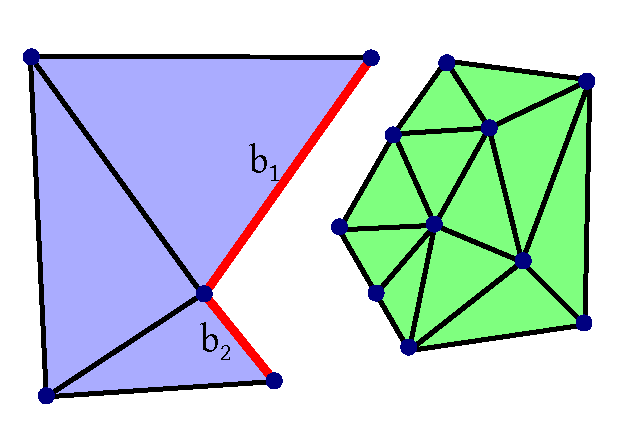
\includegraphics[width=0.475\textwidth]{./img/ch-incr-dens/meshmerge03new}&
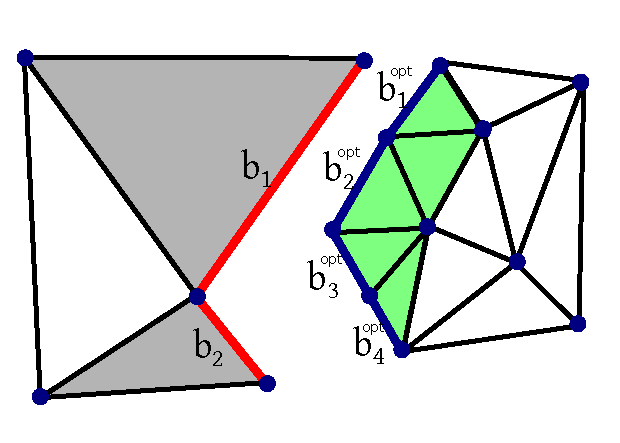
\includegraphics[width=0.475\textwidth]{./img/ch-incr-dens/meshmerge04new}\\
(c)&(d)\\
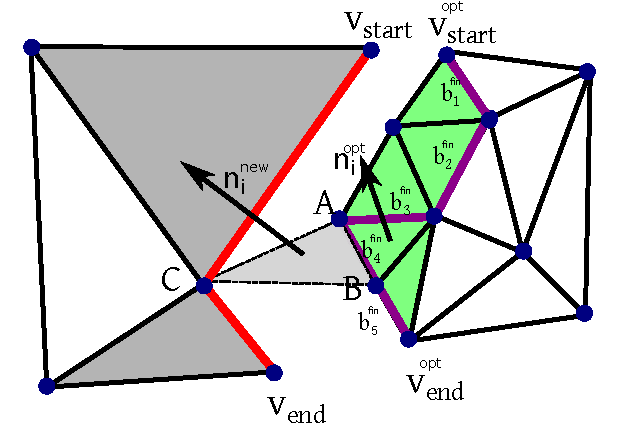
\includegraphics[width=0.475\textwidth]{./img/ch-incr-dens/meshmerge05new}&
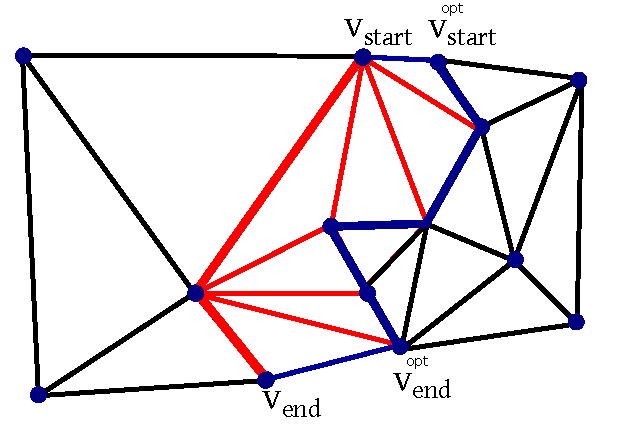
\includegraphics[width=0.475\textwidth]{./img/ch-incr-dens/meshmerge06new}\\
(e)&(f)\\
\end{tabular}
\caption{Mesh merging steps}
\label{fig:mesh_merging}
\end{figure}

We build the bounding boxes around the facets of the two meshes, and we detect which box from the refined mesh intersect a box from the new mesh, as the red boxes in Figure \ref{fig:mesh_merging}(b); then, we remove the corresponding facets as in Figure \ref{fig:mesh_merging}(c).

Once the facets have been removed, $\mathit{M}$ splits into a set of connected submeshes; we select the biggest submesh, named  $\mathit{{M}_{big}}$.
We order the edges of boundary of $\mathit{{M}_{big}}$ into a list $\mathit{b} = \{b_1, \dots,  b_n\}$.
Let $T_{\text{init}}$ be the number of the triangle of  $\mathit{M}$; if the triangles of $\mathit{{M}_{big}}$ are lower than a threshold $\tau_{bm}=30\% (T_{\text{init}})$, it means that the overlapping with the refined mesh is predominant and we stop the merging process, keeping the refined mesh as output.

If the process continues, we retrieve the set of bounding boxes around the facets adjacent to the border $\mathit{b}$, \ie, the gray facets in Figure \ref{fig:mesh_merging}(d), and we find the set $\mathit{F}^{\text{opt}}$ of facets  belonging to the refined mesh which intersects these bounding boxes, \eg, the green facets  in Figure \ref{fig:mesh_merging}(d).
The boundary edges of $\mathit{F}^{\text{opt}}$ populate the list  $\mathit{b}^{\text{opt}} = \{b_1^{\text{opt}}, \dots,  b_m^{\text{opt}}\}$, and, among these edges, we select the vertices  $v_{\text{start}}^{\text{opt}}$ and $v_{\text{end}}^{\text{opt}}$ which are the vertices nearest to the extremity $v_{\text{start}}$ and  $v_{\text{end}}$ of the boundary $\mathit{b}$ (see Figure \ref{fig:mesh_merging}(e)). 
We estimate the path  $\mathit{b}^{\text{fin}}$ from $v_{\text{start}}^{\text{opt}}$ to $v_{\text{end}}^{\text{opt}}$ among the edges of the facets  $\mathit{F}^{opt}$ such that it minimizes the energy:
\begin{equation}
  E_{\text{path}} = \sum_i E(b_i^{\text{opt}})= \sum_i \angle (\overrightarrow{n}_i^{\text{opt}},\overrightarrow{n}_i^{\text{new}})
\end{equation}
where $\overrightarrow{n}_i^{\text{opt}}$ is the normal of the facet among $\mathit{F}^{opt}$ adjacent to  $b_i^{\text{opt}}$; and
$\overrightarrow{n}_i^{\text{new}}$ is the normal of the facet defined by the two extremities $A$ and $B$ of edge ${b}^{\text{opt}}$ and the nearest vertex $C \in \mathit{b}$.
We minimize $E_{\text{path}}$ with the Dijkstra algorithm  and we extract the final boundary $\mathit{b}^{\text{fin}} = \{ b_1^{\text{fin}}, \dots, b_s^{\text{fin}}\}$ (Figure \ref{fig:mesh_merging}(e)).

Finally, we connect $v_{\text{start}}^{\text{opt}}$ to $v_{\text{start}}$  and $v_{\text{end}}^{\text{opt}}$ to  $v_{\text{end}}$ such that we create a closed polyline $\{v_{\text{start}}^{\text{opt}},  v_{\text{start}}, \mathit{b}, v_{\text{end}}^{\text{opt}}, v_{\text{end}}, \mathit{b}^{\text{fin}}\}$, that we fill with the manifold-preserving algorithm proposed in \cite{liepa2003filling}  (Figure \ref{fig:mesh_merging}(f)). 
To handle the possible topology change of the mesh, we iterate this process for all the boundaries of the mesh  $\mathit{\bar{M}}_{0..kW}$, not negligible, \ie, smaller than $\tau_{\text{top}}= 15\%$ the biggest boundary.

The final mesh $\mathit{M}^{\text{merged}}$ is composed by all the facets from the refined mesh $\mathit{M}^{\text{opt}}$ which have not been removed by the previous process, the submeshes kept from the new mesh $\mathit{M}$ and finally the facets created to fill the polylines.



\section{Experimental Evaluation}
\label{sec:exp}
We tested the proposed system in order to stress the flexibility of the approach both for small objects and for large-scale scenes.
In these experiments we used two classical \mvs datasets to test the generality of our approach with  images that do not comes from a video  sequence; we therefore cannot apply the Edge-Point reconstruction which rely on feature tracking. 
Therefore, we bootstrap our algorithm from the points, cameras and visibility rays extracted by the incremental pipeline provided by openMVG \cite{openMVG}. 
In Table \ref{fig:expData} we list the features of each dataset, and the statistics of the reconstruction: number of reconstructed surfaces, number of mesh merging steps and window size, which is chosen to stress the iterative nature of the proposed algorithm.
We performed the experiments on a 4 Core i7-920 CPU at 2.6Ghz (8M Cache), with 16GB of DDR3 SDRAM and a GPU Nvidia GT630M.


\begin{table}[t]
\normalsize
\centering
\setlength{\tabcolsep}{1px}
  \caption{Output statistics on the two datasets.}
  \label{fig:expData}
\begin{tabular}{lccccc}
&num. cameras& resolution&num. facets& num. merged &$W$ \\
\hline
dinoRing&48&640x480&$\sim$127K&3&15\\
castle P-18&18&3072x2048&$\sim$4.7M&3&5\\
\end{tabular}
\end{table}

In the first experiment, we tested our approach with the \emph{dinoRing} dataset  from the Middelbury evaluation proposed in \cite{seitz2006comparison}. 
The dataset is composed by 48 640x480 images; in Table \ref{tab:dinoRes} we report the comparison with the top ranked algorithm \cite{savinov2016semantic}, which is voxel-based, together with the other mesh-based algorithm closer to our proposal.
Our algorithm reaches a less accurate result, but  the output is comparable with batch state-of-the art algorithms, despite two big restrictions we are forced to work with.
First, our algorithm is the only technique  which estimate incrementally the surface; it considers the images as a sequence and compares only subsequent images, \ie, image $k$ with image $k-1$.
Second, we cannot exploit any silhouette information, and the visuall hull, since it cannot be estimated in general scenes.

Figure \ref{fig:dinoIncr} illustrates the incremental reconstruction of dino: the red circles underline the topology changes handled by our mesh merging algorithm.

\begin{table}[t]
\normalsize
\centering
\setlength{\tabcolsep}{1px}
  \caption{Results on dinoRing dataset.}
  \label{tab:dinoRes}
    \begin{tabular}{lcccccc}
    %method & Accuracy (mm) &Completeness (\%)\\
    \hline
    &
    %Savinov
    \cite{savinov2016semantic}&
    %DCV
    \cite{li2015detail}&
    %Zarahescu
    \cite{zaharescu2007transformesh}&
    %Vu
    \cite{hiep2009towards}&%SurfEvolution&
    %Gargallo
    \cite{gargallo2007minimizing}&proposed\\
    &(batch)&(batch)&(batch)&(batch)&(batch)&%(batch)&
    (incremental)\\
    \hline
    Accuracy (mm) &0.25&0.28&0.42&0.53&%0.56&
    0.6&1.27\\
    Comp. (\%)&99.9&100&98.6&99.7&%97.7&
    92.9&87.8
    \end{tabular}
\end{table}



\begin{sidewaysfigure}
% \begin{landscape}
%  \begin{figure}[t]
  \centering
  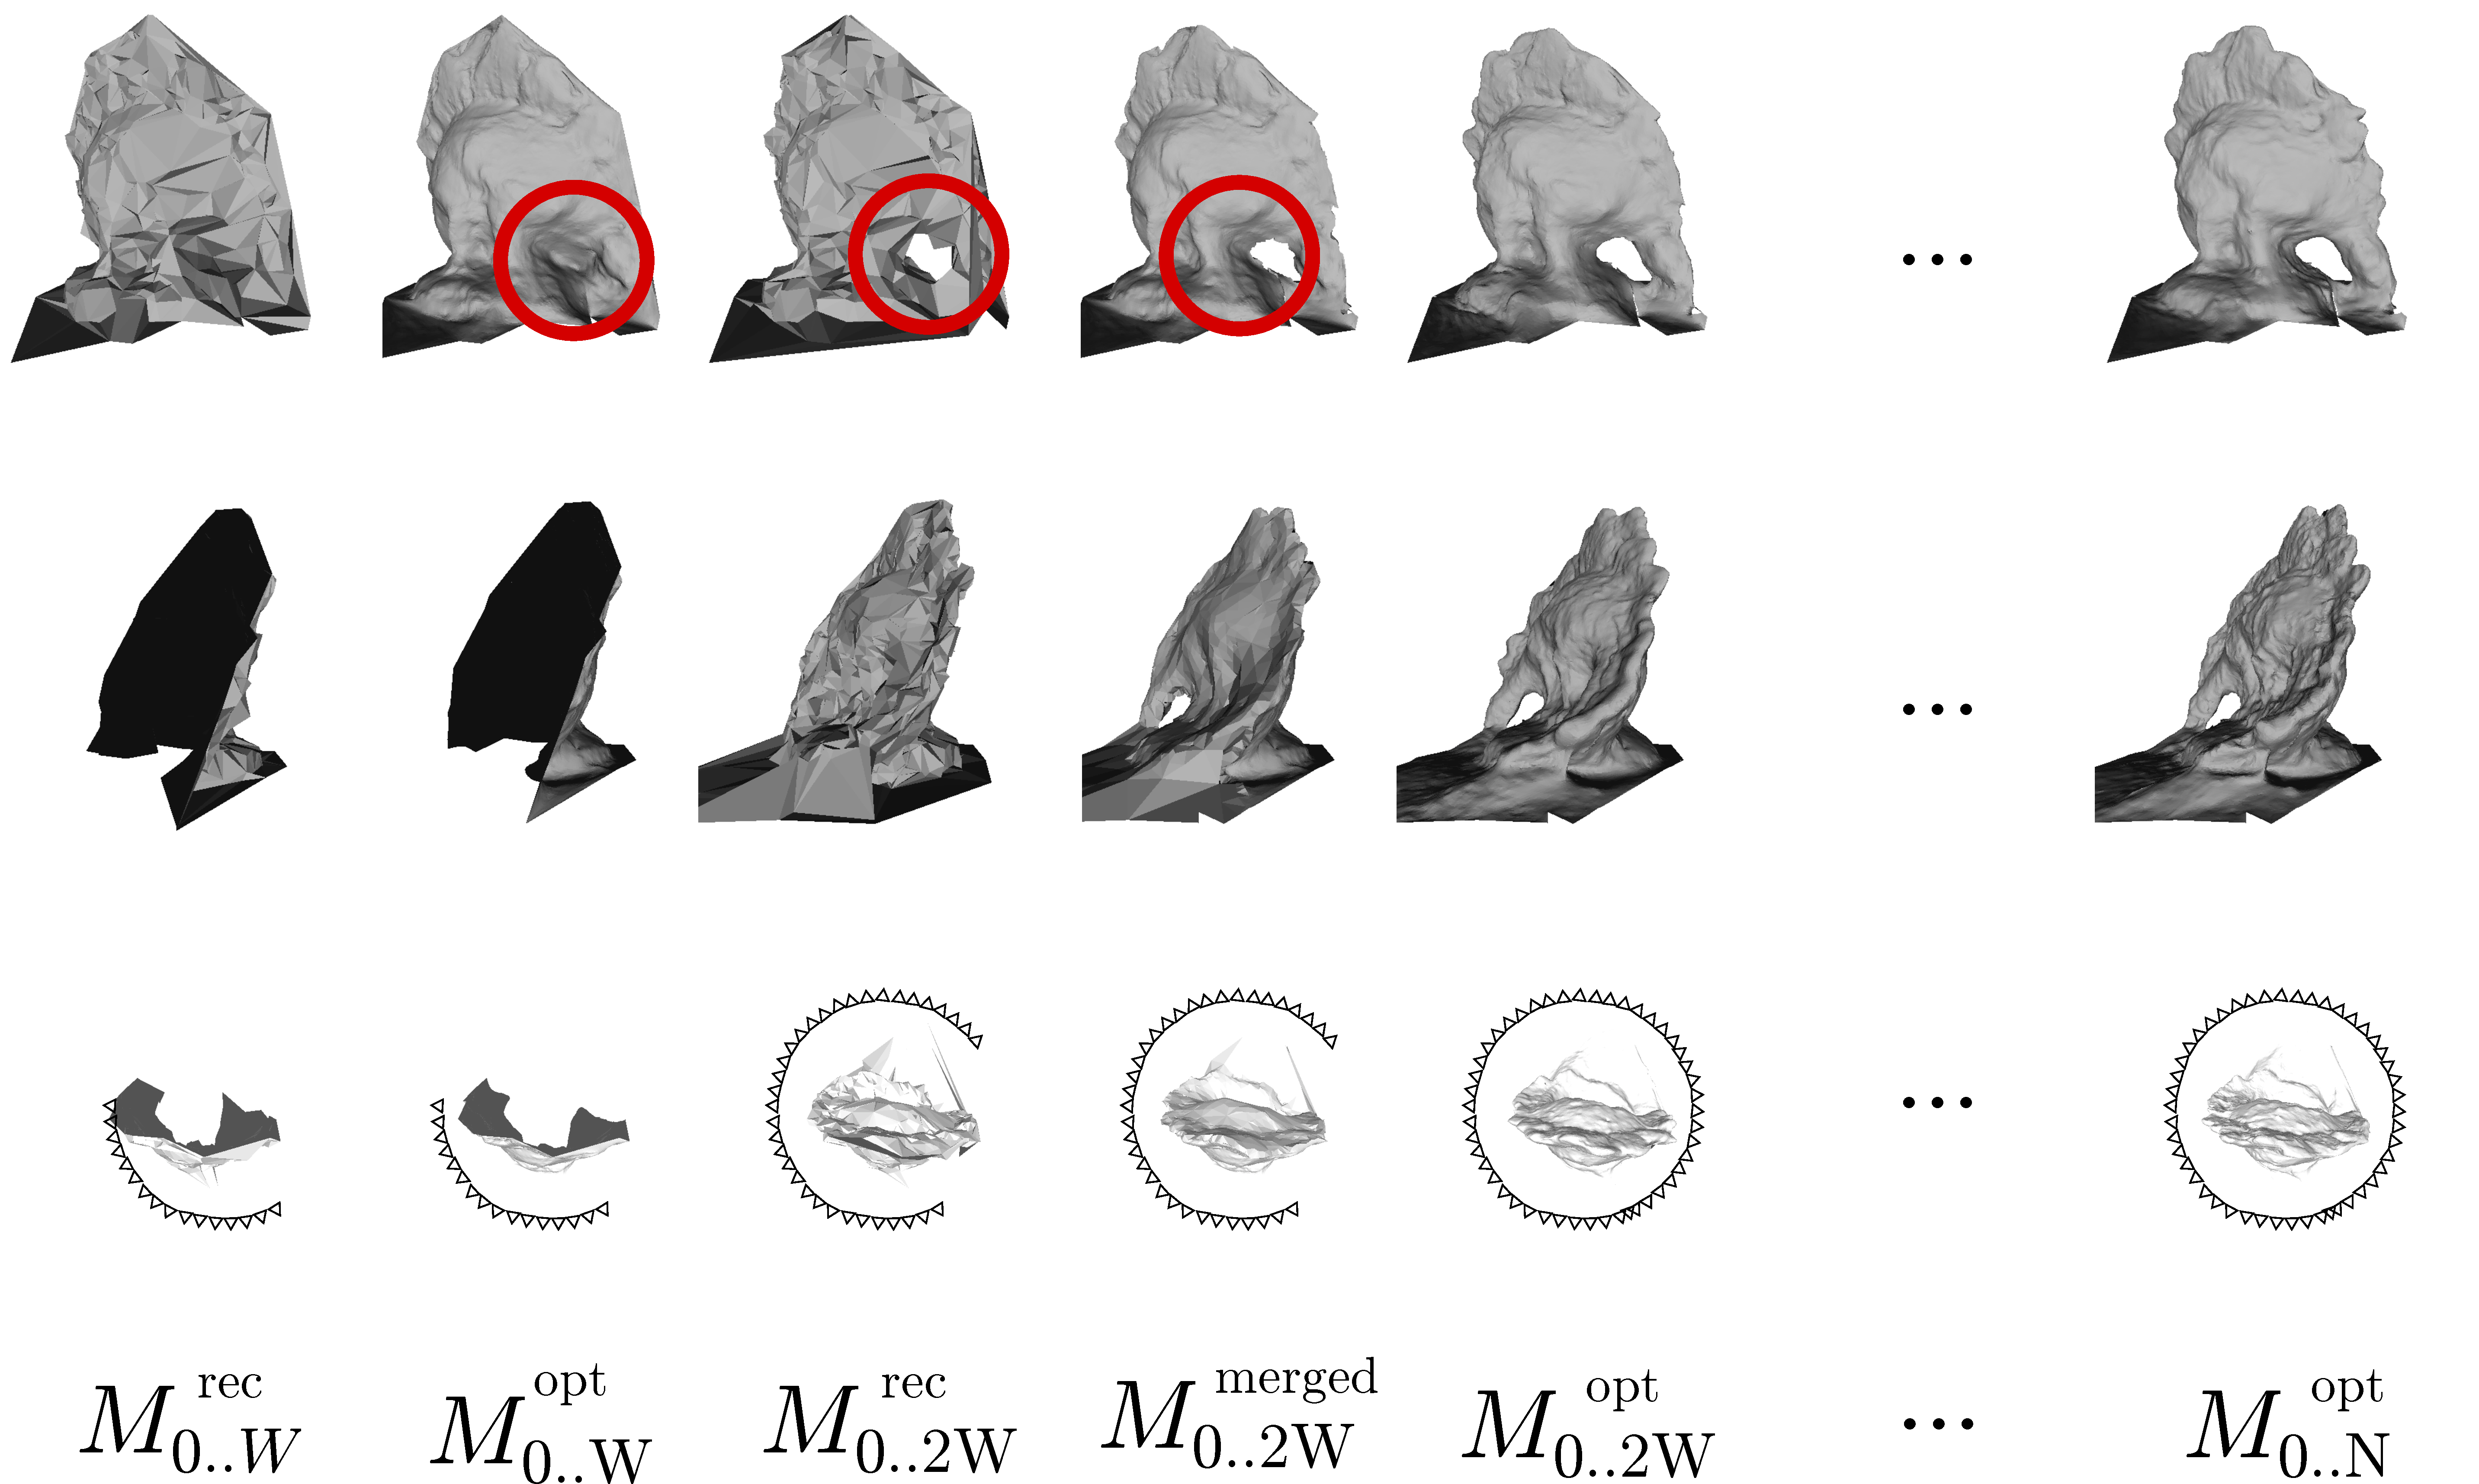
\includegraphics[width=\textwidth]{./img/ch-incr-dens/dino}
  \caption{Incremental reconstruction on the dino dataset.}
  \label{fig:dinoIncr}
% \end{figure}
% \end{landscape}
\end{sidewaysfigure}


Then we experimented our approach with the \emph{castle-P18} dataset provided in \cite{strecha2008} (Figure \ref{fig:castleOriginal}); no ground truth is available, but it is the only sequence of the dataset able to show the incremental behavior of our approach, since subset of cameras observe parts of the scene. 
The Figure \ref{fig:castle} shows the results, and Figure \ref{fig:detailcastle} displays details of the reconstruction before and after the refinement. The final reconstruction is accurate  an detailed, especially with respect to the initial rough mesh.
Let notice in Table \ref{fig:expData} that the number of the reconstructed facet is huge, but all the computations have been performed in memory without the need to dump any data on disk. Indeed the volumetric stage of our algorithm, \ie, the incremental manifold reconstruction, extracts only a  simplified mesh, which is successively refined relying on a mesh-based representation.


\begin{figure}[tbhp]
\centering
\setlength{\tabcolsep}{1px}
\begin{tabular}{cc}
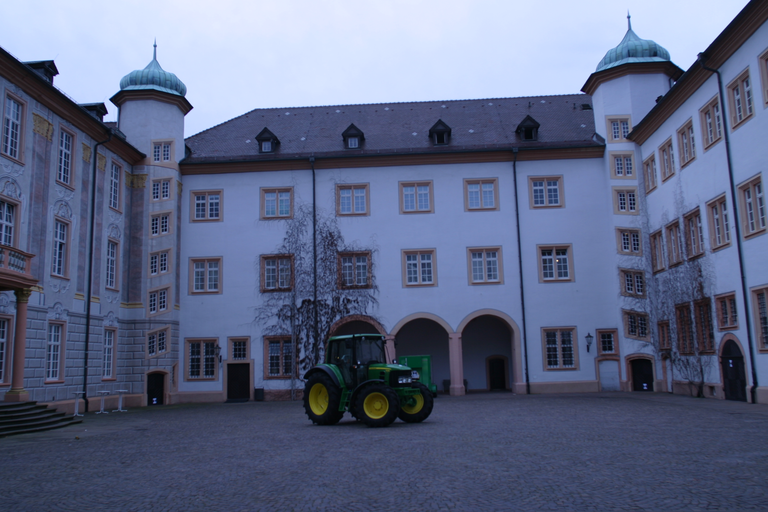
\includegraphics[width=0.4\textwidth]{./img/ch-incr-dens/castle/0000_smal}&
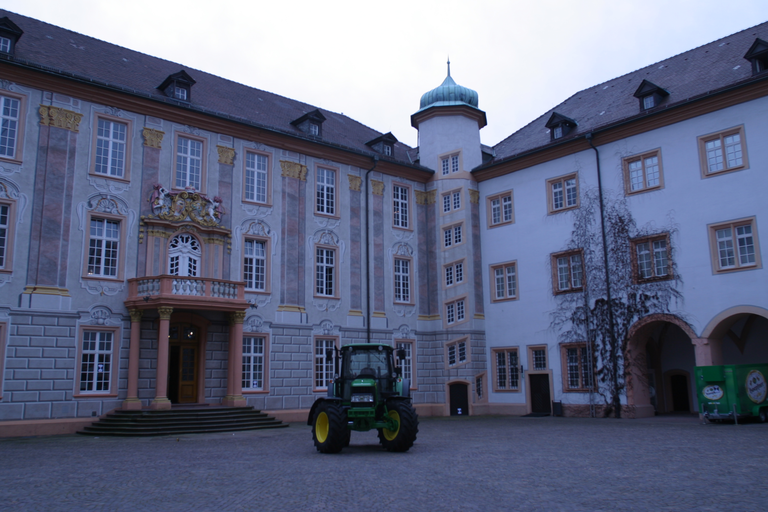
\includegraphics[width=0.4\textwidth]{./img/ch-incr-dens/castle/0003_smal}\\
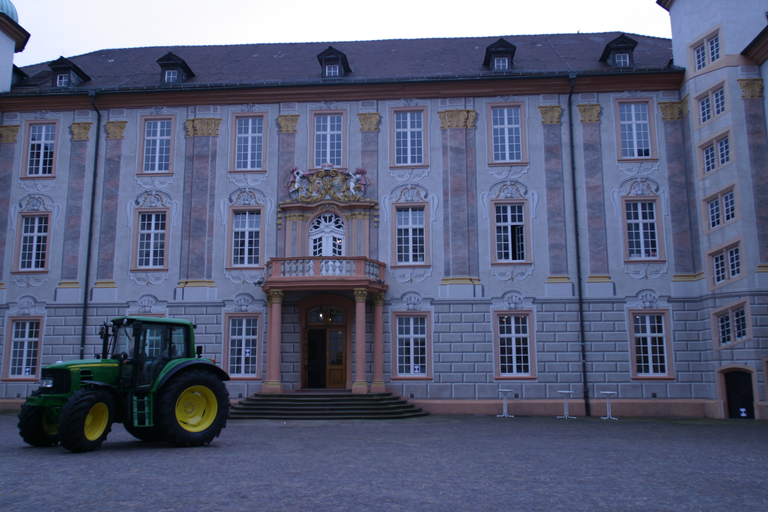
\includegraphics[width=0.4\textwidth]{./img/ch-incr-dens/castle/0006_smal}&
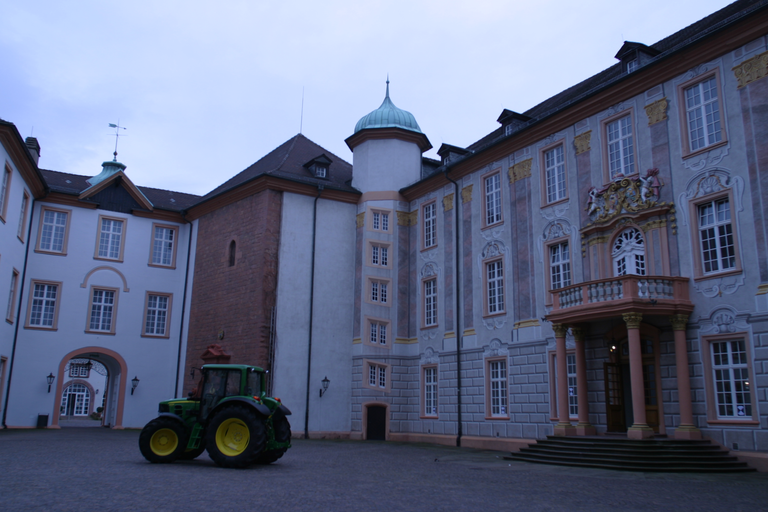
\includegraphics[width=0.4\textwidth]{./img/ch-incr-dens/castle/0009_smal}\\
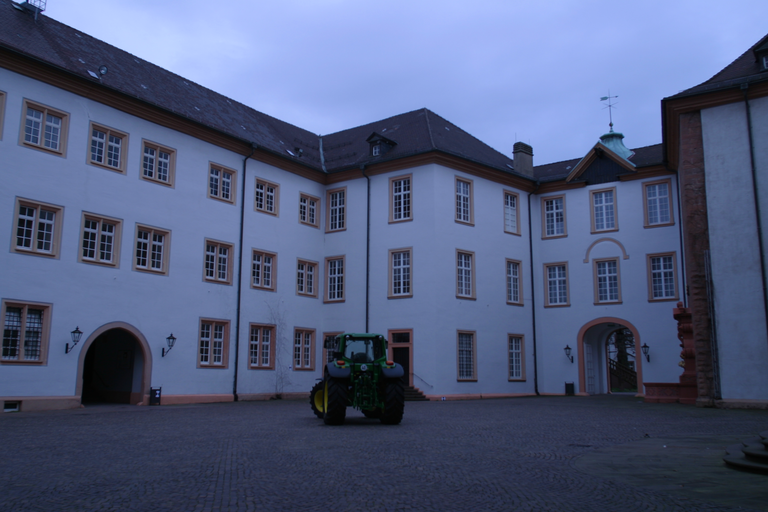
\includegraphics[width=0.4\textwidth]{./img/ch-incr-dens/castle/0012_smal}&
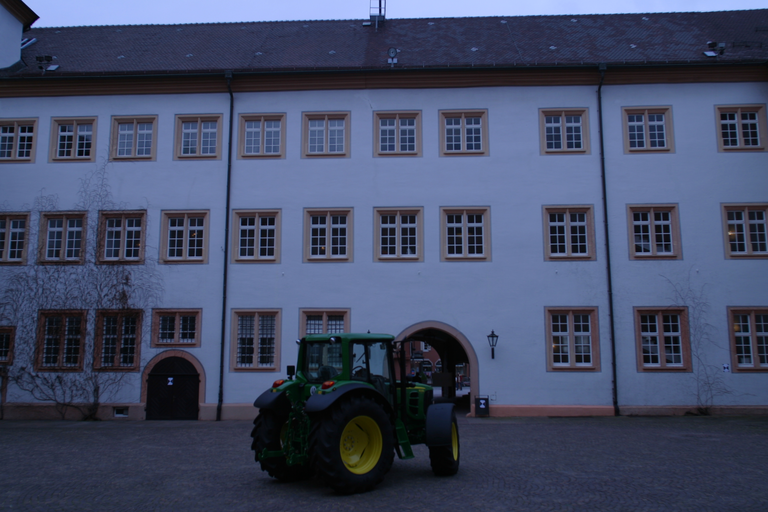
\includegraphics[width=0.4\textwidth]{./img/ch-incr-dens/castle/0015_smal}\\
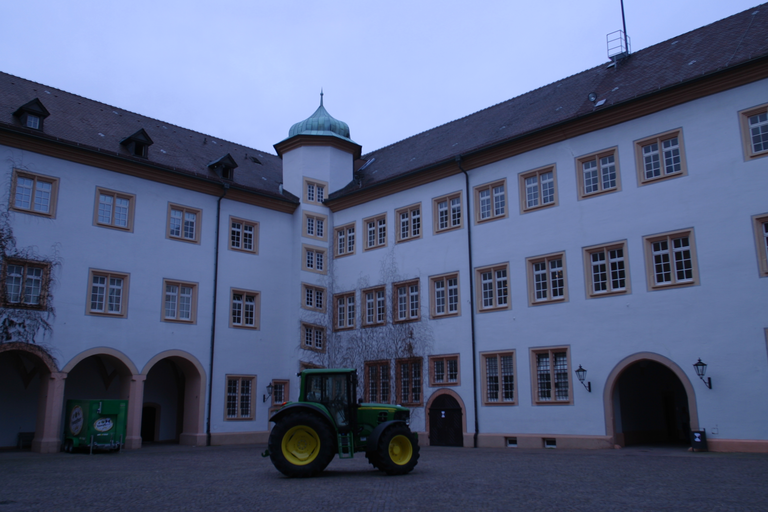
\includegraphics[width=0.4\textwidth]{./img/ch-incr-dens/castle/0017_smal}&
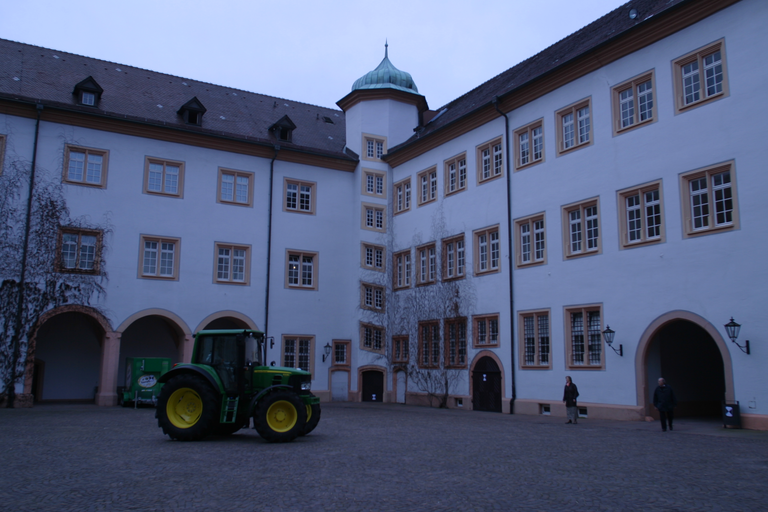
\includegraphics[width=0.4\textwidth]{./img/ch-incr-dens/castle/0018_smal}\\
\end{tabular}
\caption{Images of \emph{castle-P18} dataset}.
\label{fig:castleOriginal}
\end{figure}



\begin{figure}[t]
\centering
\setlength{\tabcolsep}{1px}
\begin{tabular}{c}
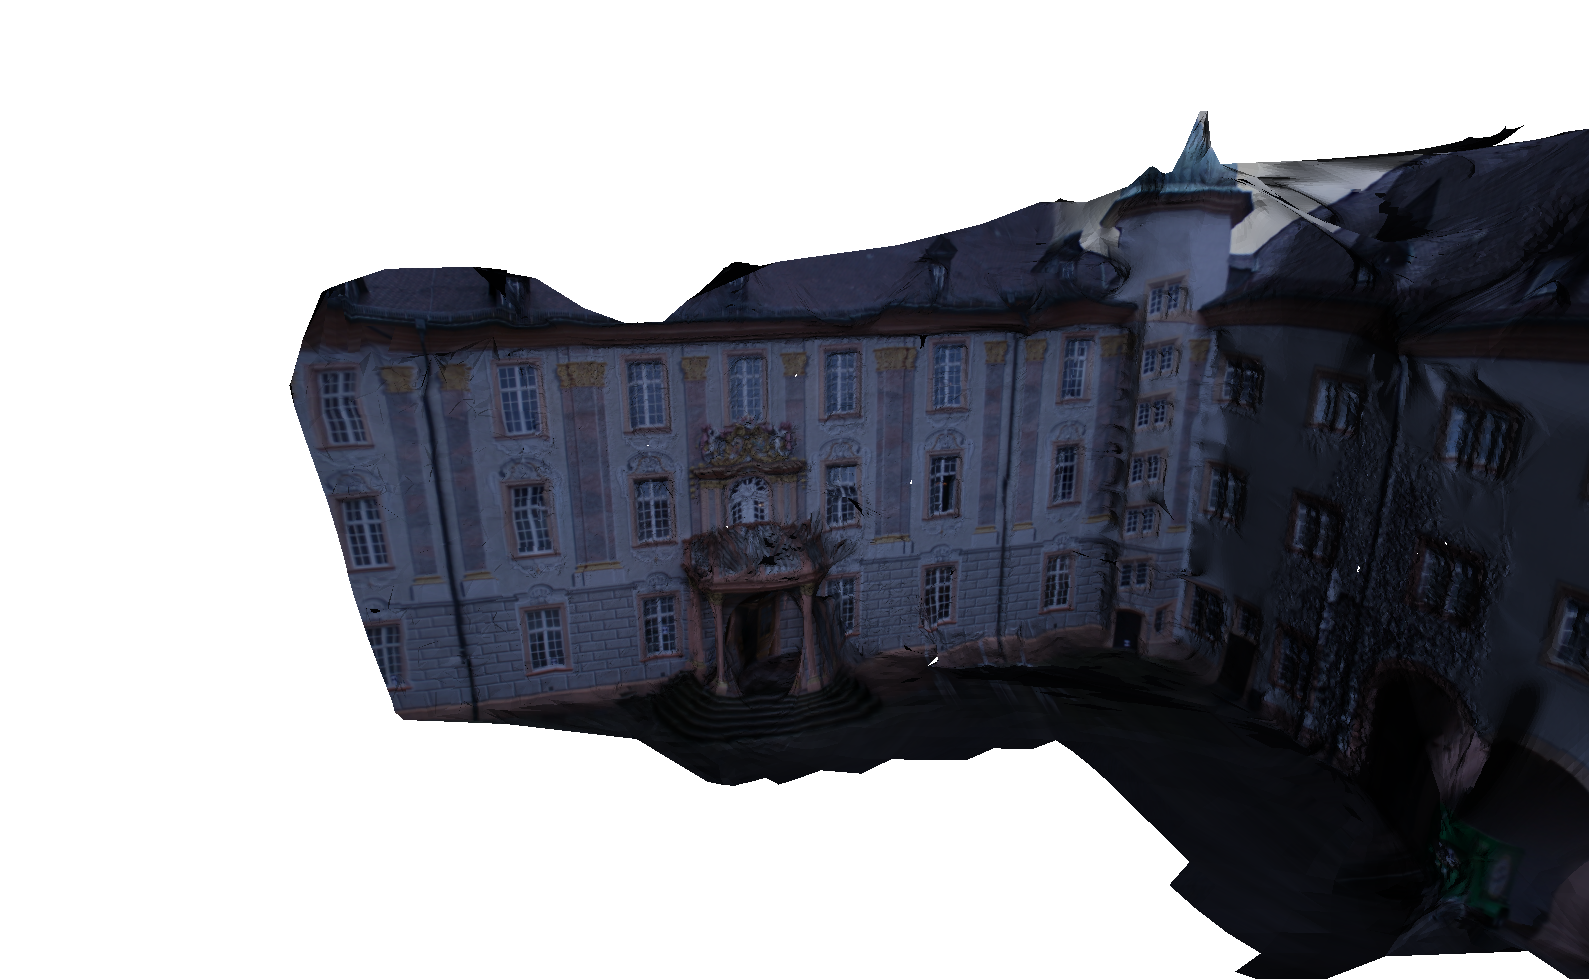
\includegraphics[width=0.6\textwidth]{./img/ch-incr-dens/castle01}\\
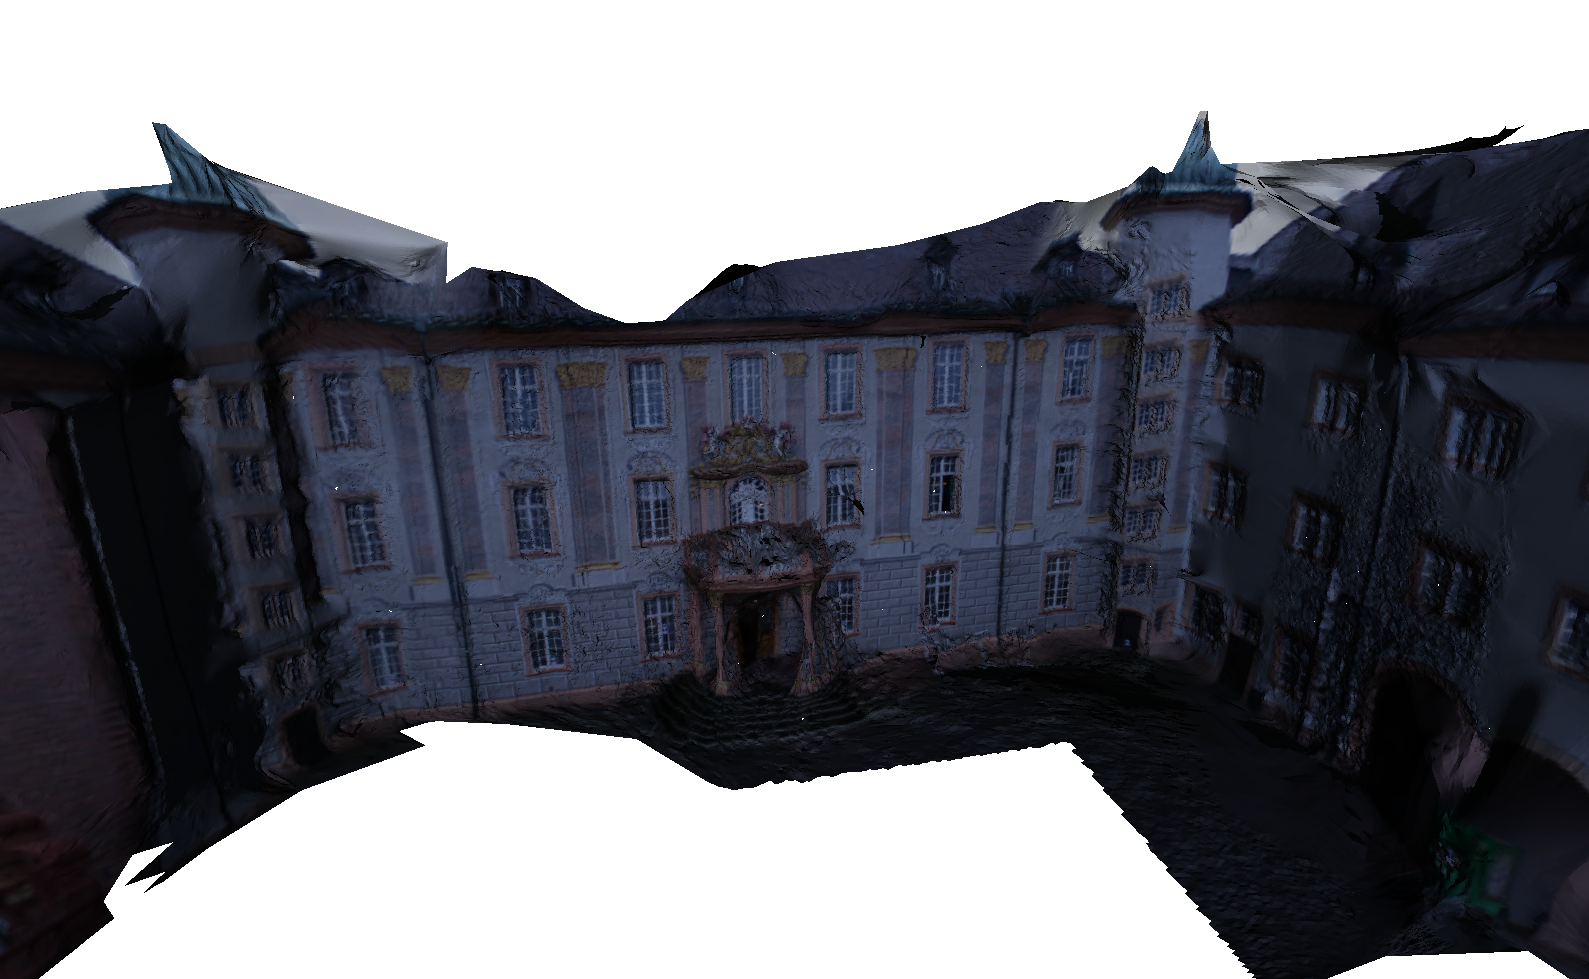
\includegraphics[width=0.6\textwidth]{./img/ch-incr-dens/castle02}\\
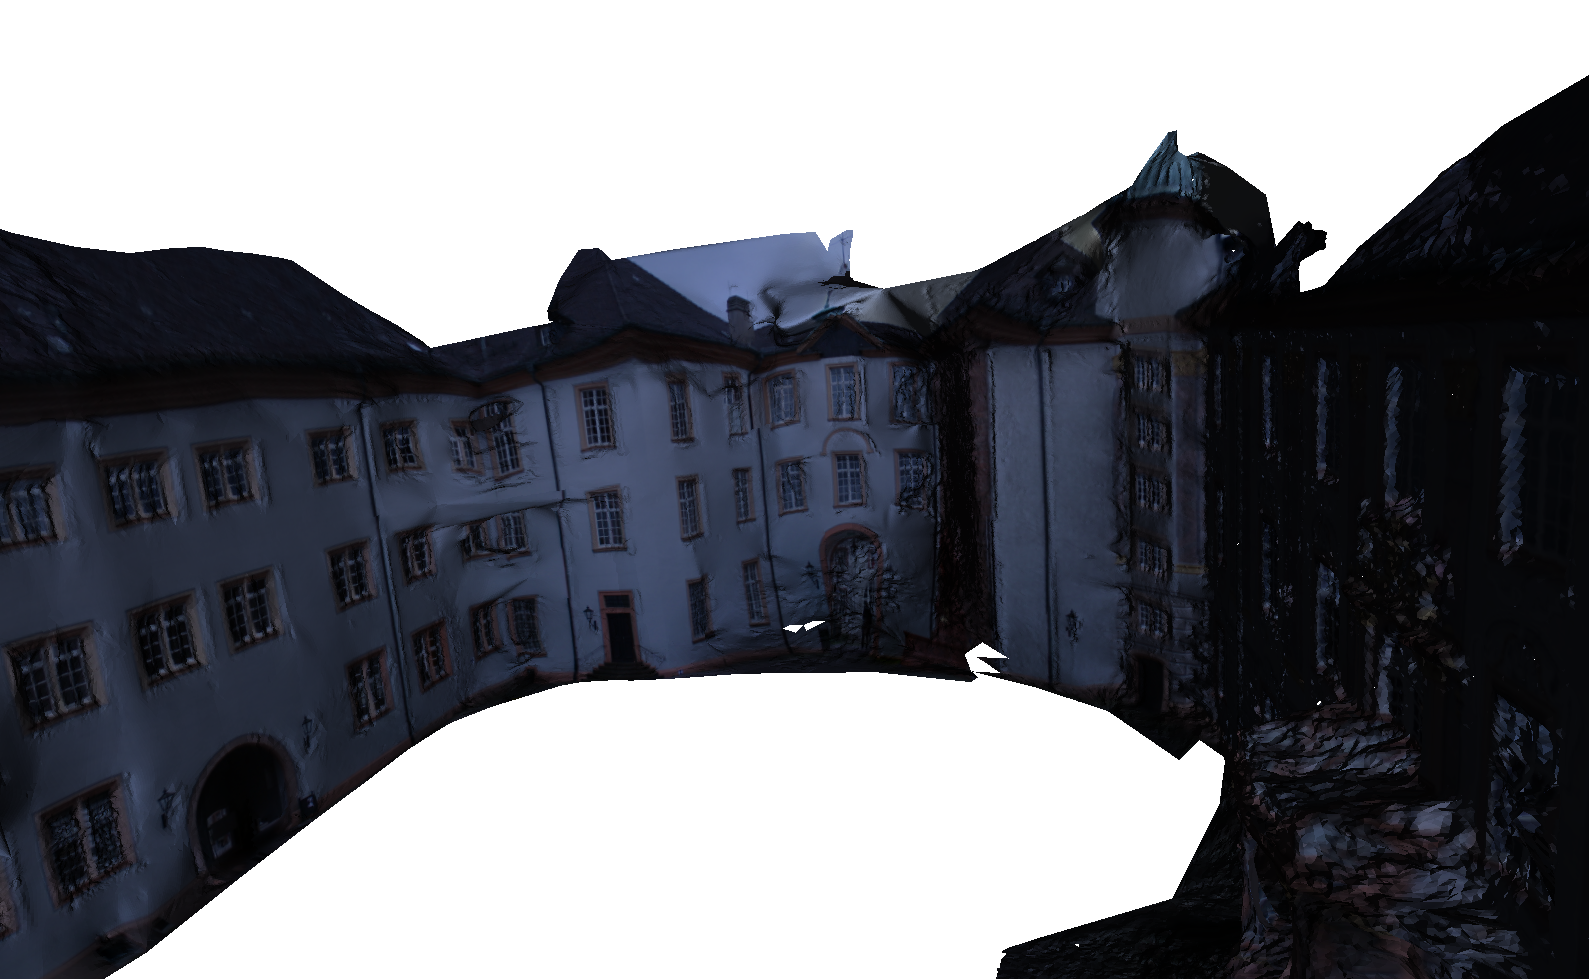
\includegraphics[width=0.6\textwidth]{./img/ch-incr-dens/castle03}\\
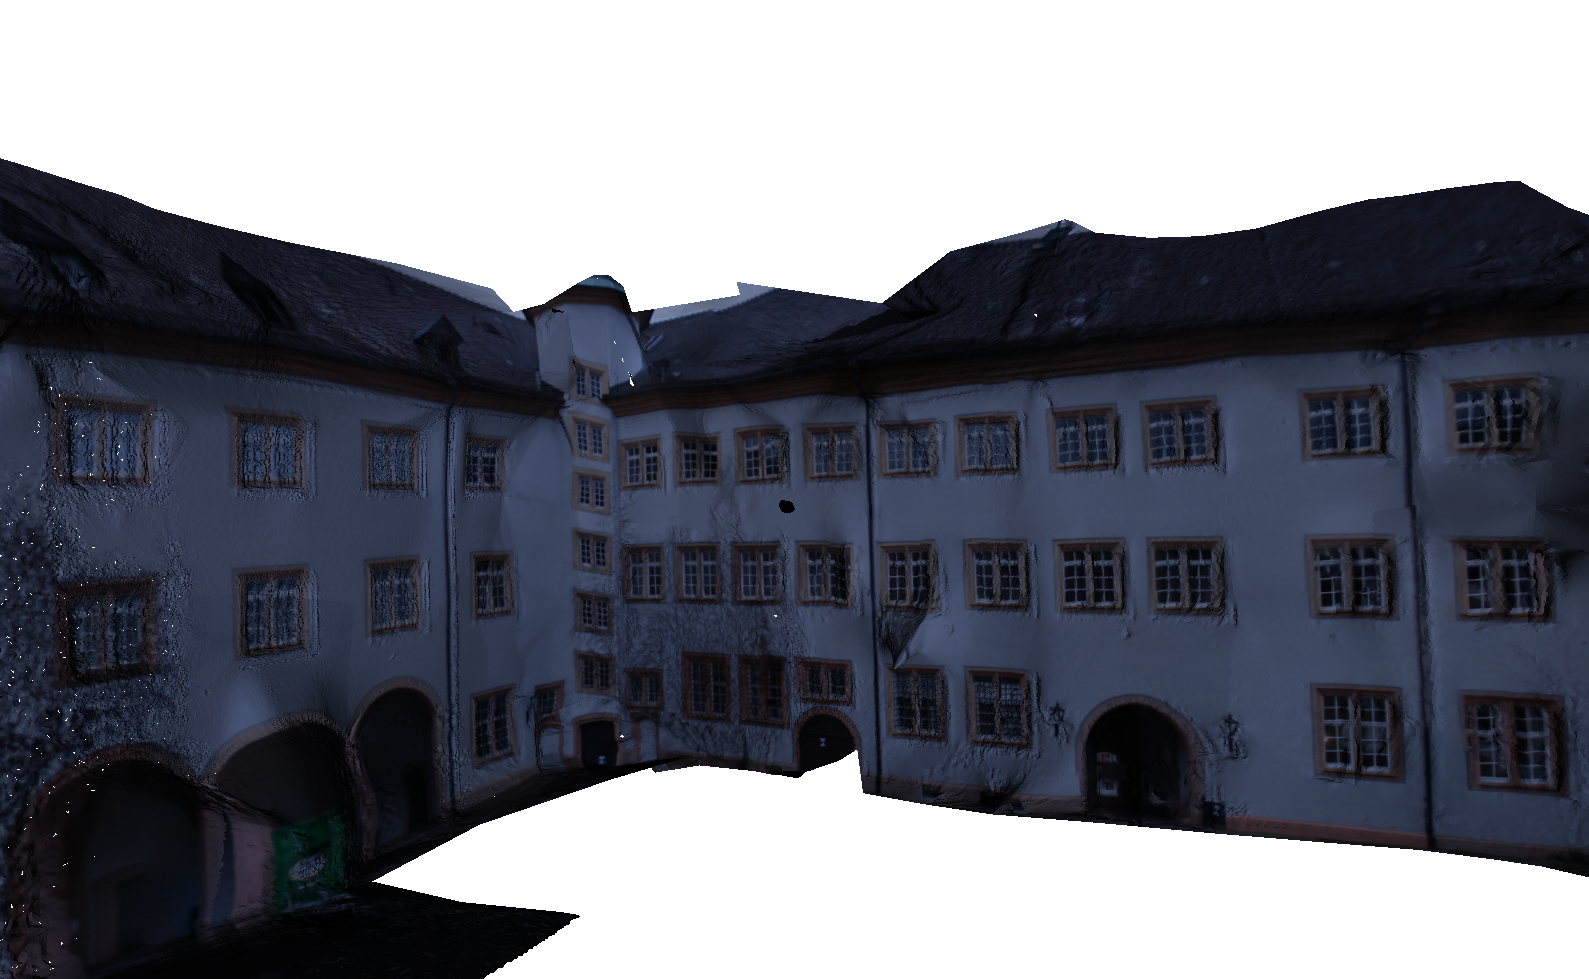
\includegraphics[width=0.6\textwidth]{./img/ch-incr-dens/castle04}
\end{tabular}
\caption{Incremental reconstruction of \emph{castle-P18} dataset}.
\label{fig:castle}
\end{figure}

\begin{figure}[tp]
\centering
\setlength{\tabcolsep}{1px}
\begin{tabular}{cc}
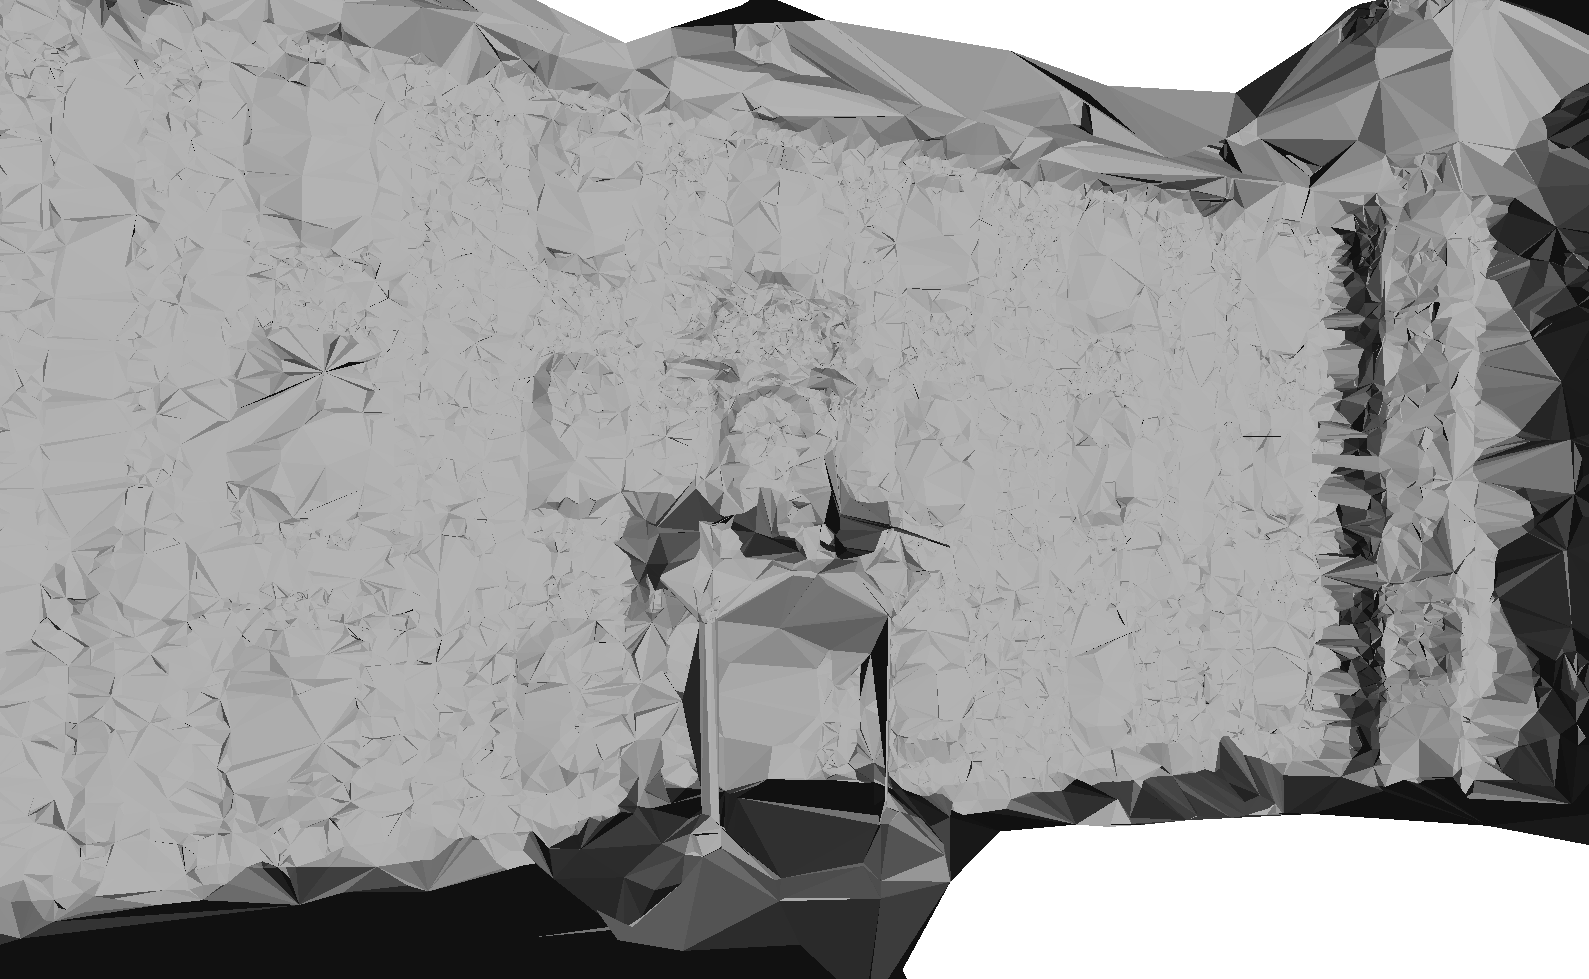
\includegraphics[width=0.48\textwidth]{./img/ch-incr-dens/castle05}&
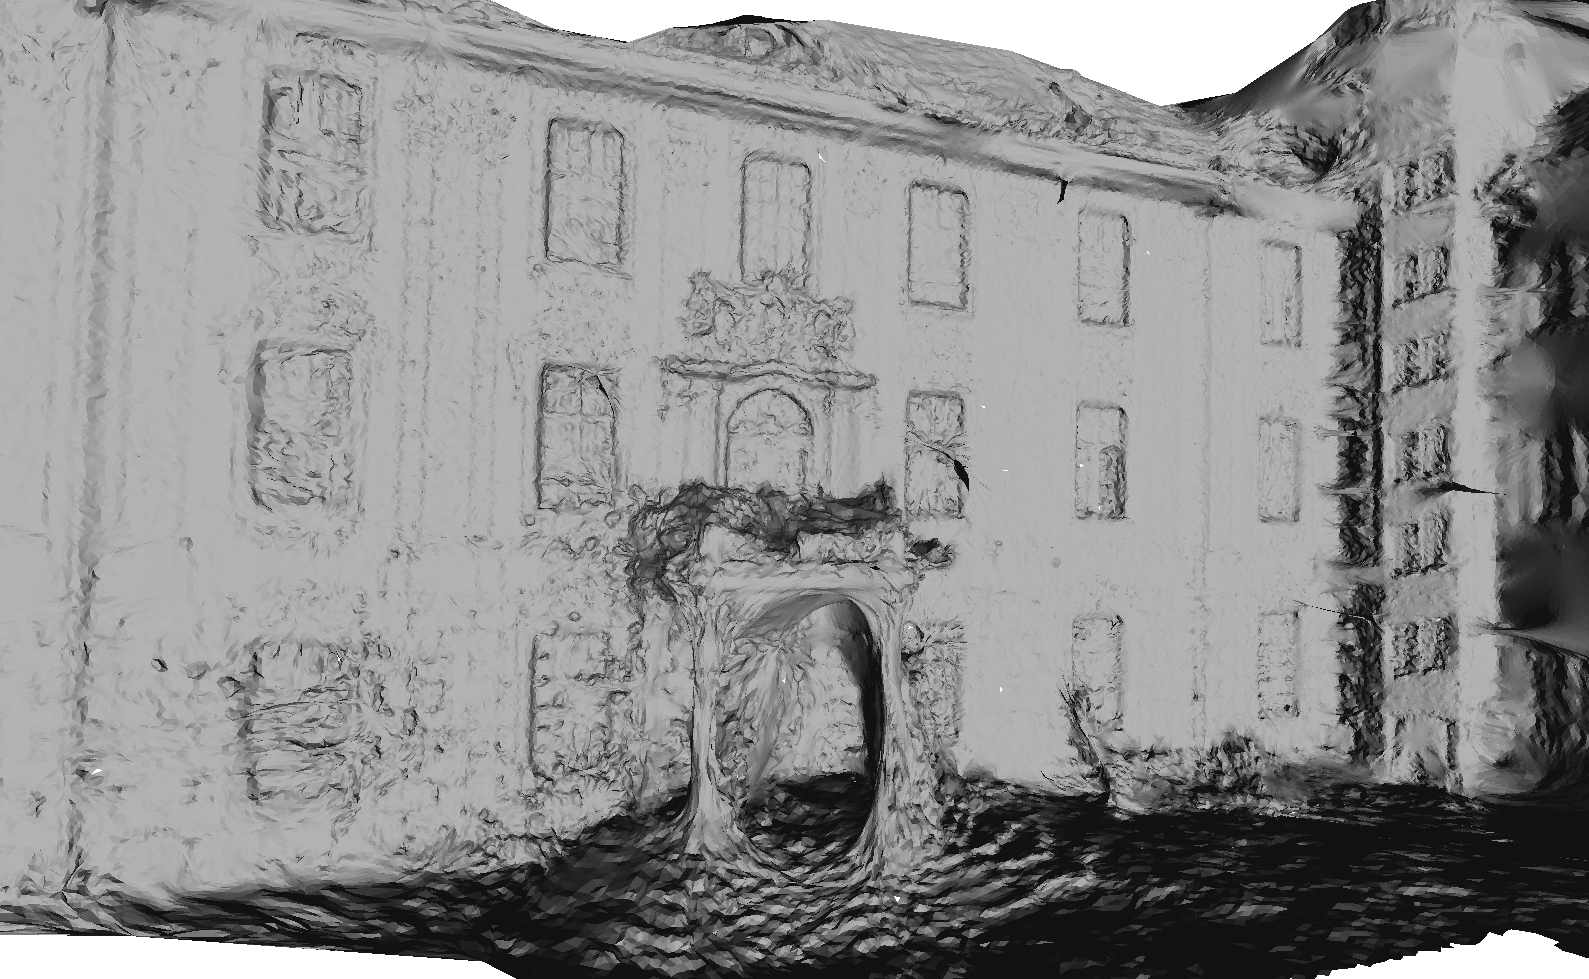
\includegraphics[width=0.48\textwidth]{./img/ch-incr-dens/castle06}\\
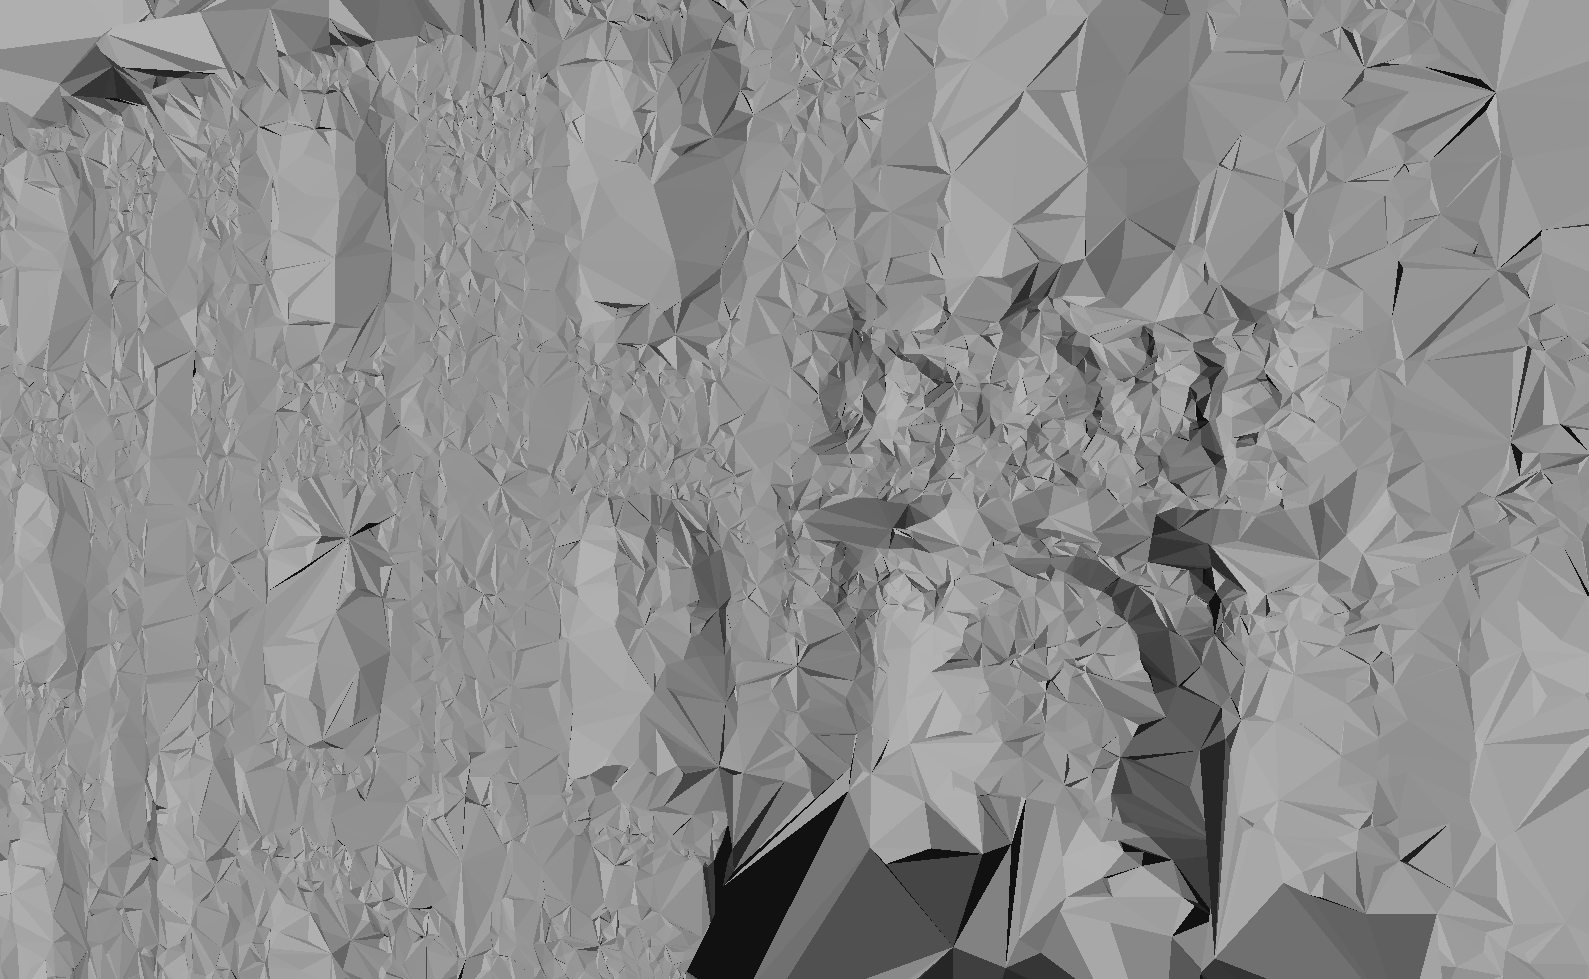
\includegraphics[width=0.48\textwidth]{./img/ch-incr-dens/castle07}&
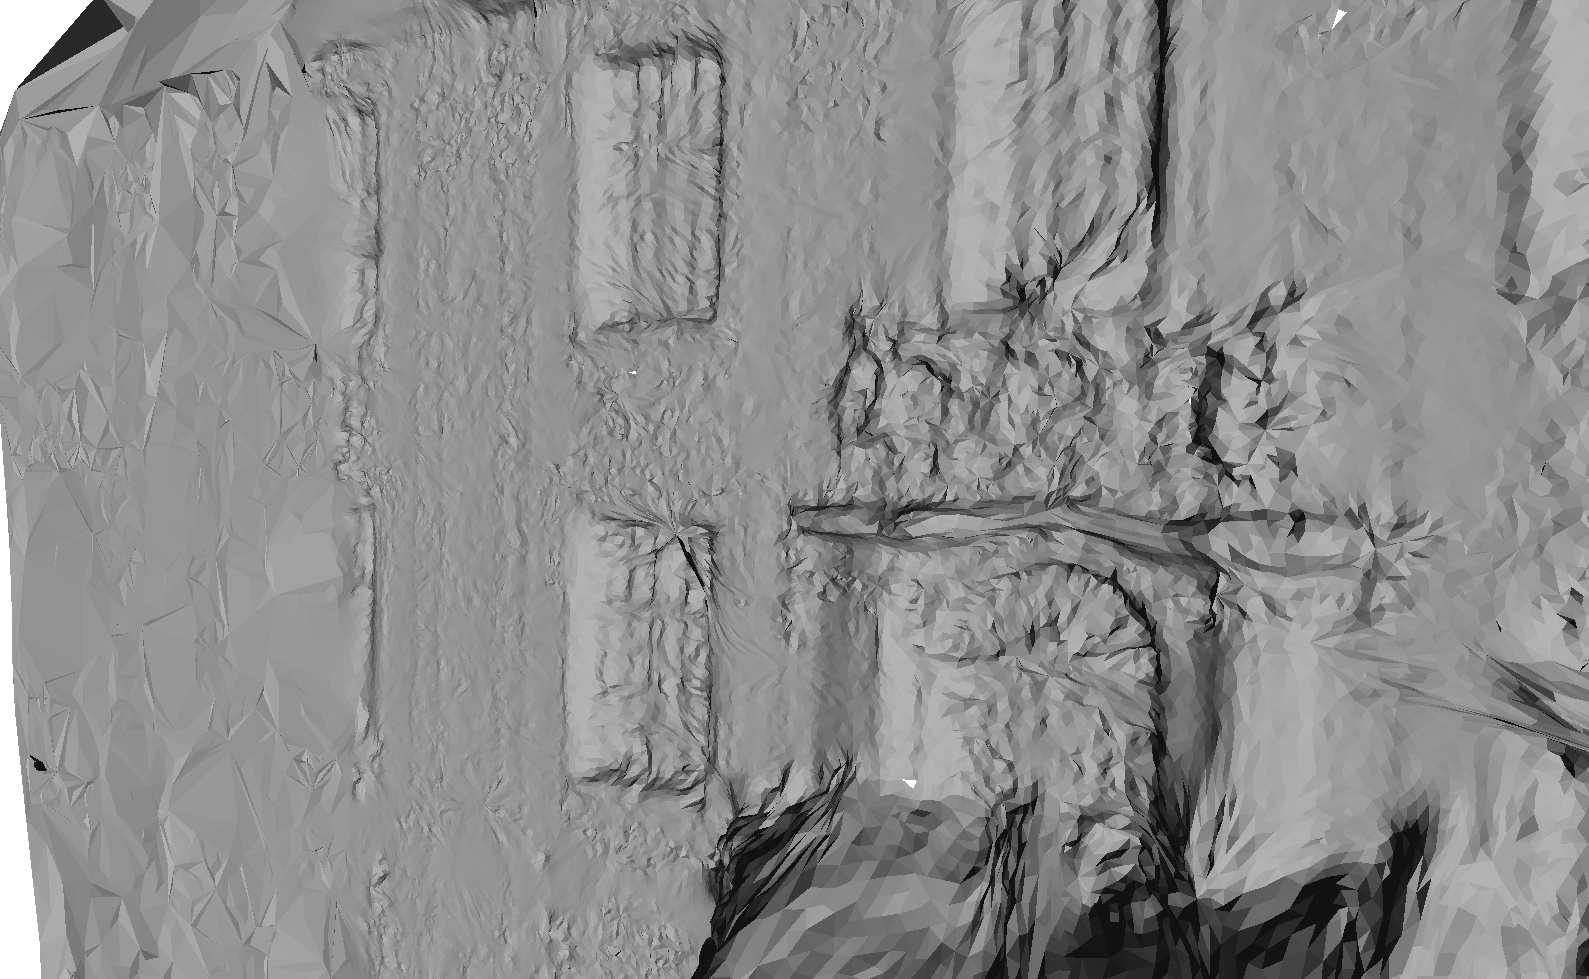
\includegraphics[width=0.48\textwidth]{./img/ch-incr-dens/castle08}\\
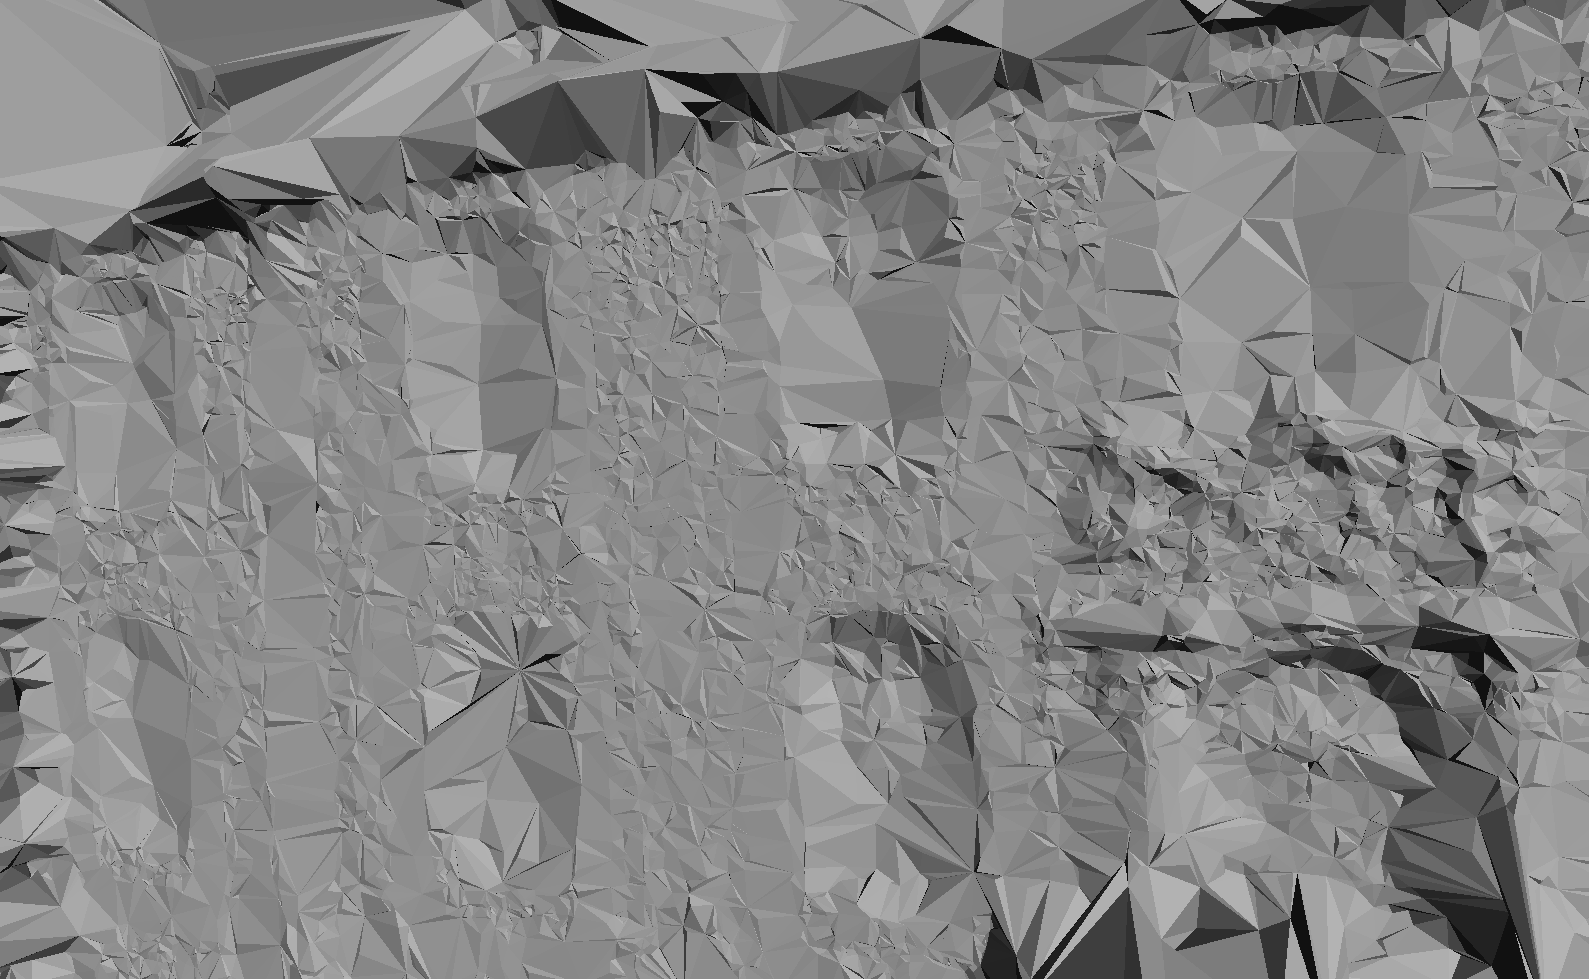
\includegraphics[width=0.48\textwidth]{./img/ch-incr-dens/castle12}&
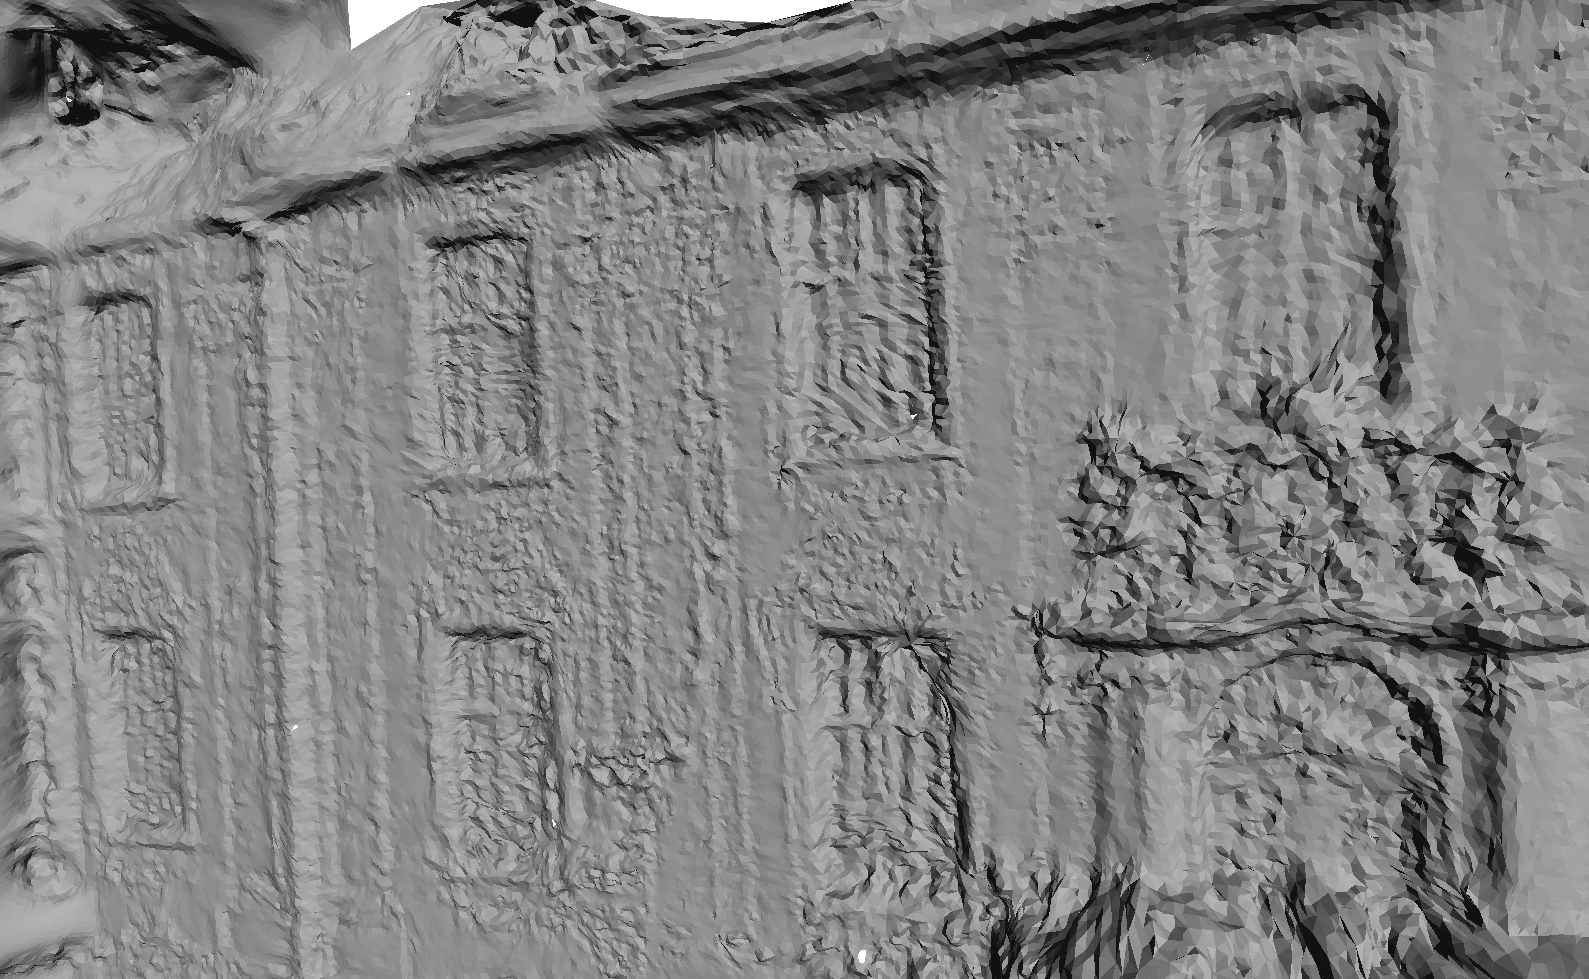
\includegraphics[width=0.48\textwidth]{./img/ch-incr-dens/castle11}\\
(a)&(b)
\end{tabular}
\caption{Detail of Castle reconstruction before (a) and after (b) the photo-metric refinement}.
\label{fig:detailcastle}
\end{figure}
% \begin{figure}[tp]
% \centering
% \setlength{\tabcolsep}{1px}
% \begin{tabular}{c}
% 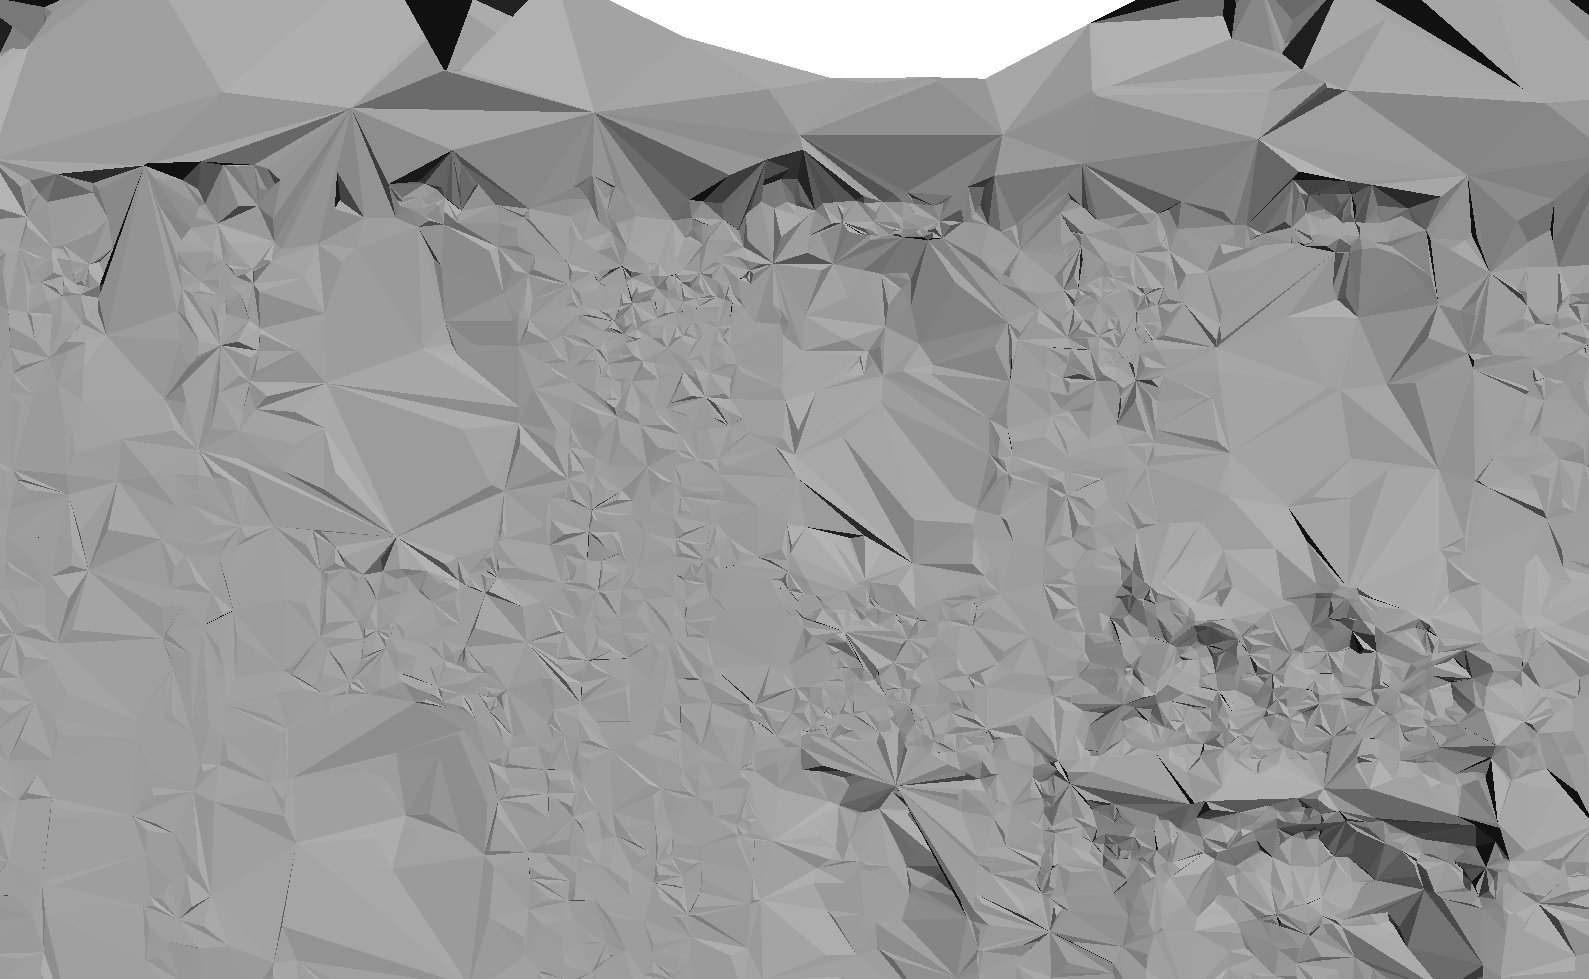
\includegraphics[width=0.92\textwidth]{./img/ch-incr-dens/castle09}\\
% (a)\\
% 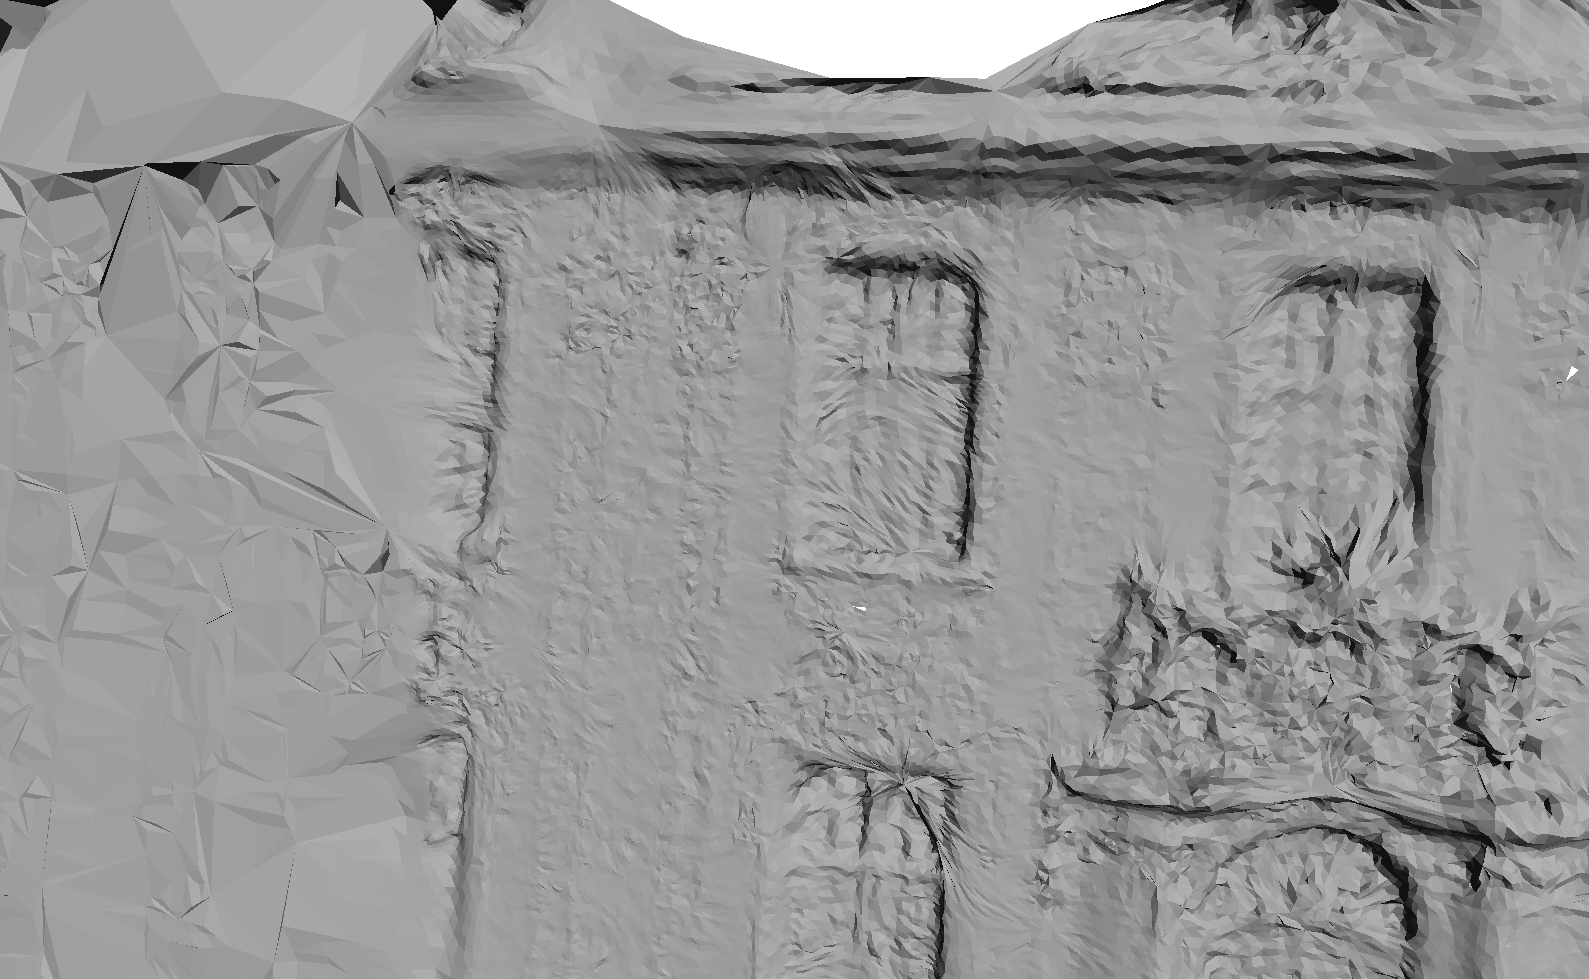
\includegraphics[width=0.92\textwidth]{./img/ch-incr-dens/castle10}\\
% (b)
% \end{tabular}
% \caption{Detail of Castle reconstruction before (a) and after (b) the photo-metric refinement in the correspondence of a merging spot.}.
% \label{fig:detailcastle2}
% \end{figure}






